%% Preamble
\documentclass[
	final,
	12pt,
	fleqn
]{masterthesis}

% Packages
\usepackage[right=6em, left=6em]{geometry}  % set up margin
\usepackage[bookmarks, final]{hyperref}     % clickable references (with file outline in .pdf)
\usepackage{titlesec}                       % part header and its text in the same page
\usepackage{amsmath}                        % equations and aligned multi-line equations
\usepackage{amssymb}                        % mathematical symbols
\usepackage[inline]{enumitem}               % inline enumeration
\usepackage{csquotes}                       % quotes
\usepackage{subcaption}                     % subfigures
\usepackage{tikz}                           % plots
\usepackage{pgfplots}
\usepackage{pgfplotstable}                  % tables from files
\usepackage{booktabs}                       % horizontal rules in tables
\usepackage{multirow}                       % span table content over multiple rows
\usepackage{tikz-qtree}                     % trees
\usepackage[title,titletoc]{appendix}       % appendices
\usepackage[ruled,vlined]{algorithm2e}      % pseudocode

% Notes to self command
\usepackage{color}
\newenvironment{nts}{\begingroup\color{red}}{\endgroup}

% Title page parameters
\title{
	From Dynamic Programming to Reinforcement Learning \\
	\large{Computational Aspects}
}
\author{Andrea Guarnore}
\advisor{Alessandro Verri}
\secondadvisor{Agnese Seminara}
\examiner{Francesca Odone}
\submitmonth{September}
\submityear{2022}

% Auxiliary stuff
% Avoid semicolon at the end of each line
\SetEndCharOfAlgoLine{}

% Functions
\SetKwProg{Function}{function}{}{end}

% Infinite loops
\SetKwProg{Loop}{loop}{}{end}

% Comments
\SetKwComment{Comment}{(}{)}
\SetCommentSty{normalshape}  % normal font for comments
  % add all global settings
% Optimal control
\newcommand\statespace{\ensuremath{\mathcal{S}}}                                % MDP tuple
\newcommand\actionspace{\ensuremath{\mathcal{A}}}
\newcommand\transition{\ensuremath{p}}
\newcommand\initialdistribution{\ensuremath{p_{0}}}
\newcommand\immediatereward{\ensuremath{r}}
\newcommand\discount{\ensuremath{\gamma}}
\newcommand\randomstate{\ensuremath{s}}                                         % random variables
\newcommand\randomaction{\ensuremath{a}}
\newcommand\randomreward{\ensuremath{r}}
\newcommand\state{\MakeLowercase{\randomstate}}                                 % value of random variables
\newcommand\action{\MakeLowercase{\randomaction}}
\newcommand\reward{\MakeLowercase{\randomreward}}
\newcommand\policy{\ensuremath{\pi}}                                            % policy
\newcommand\timestep{\ensuremath{t}}                                            % timesteps
\newcommand\horizon{\ensuremath{T}}                                             % horizon

\newcommand\return{\ensuremath{G}}                                              % return and value
\newcommand\statevalue{\ensuremath{V}}
\newcommand\actionvalue{\ensuremath{Q}}
\newcommand\script[1]{\ensuremath{^{#1}}}                                       % whether to use sub- or superscripts for policy and optimality
\newcommand\policyscript{\script{\policy}}
\newcommand\optimal{\script{*}}
\newcommand\bellmanoperator{\ensuremath{B}}                                     % Bellman operators
\newcommand\valuevector{\ensuremath{U}}

\newcommand\threshold{\ensuremath{\theta}}                                      % threshold for exact methods


% Value-based reinforcement learning
\newcommand\estimatestatevalue{\MakeUppercase{\statevalue}}                     % estimate value functions
\newcommand\estimateactionvalue{\MakeUppercase{\actionvalue}}
\newcommand\timesvisited{\ensuremath{N}}                                        % times visited a state/state-action pair

\newcommand\tderror{\ensuremath{\delta}}                                        % TD learning
\newcommand\robbinsmonro{\ensuremath{\alpha}}
\newcommand\trace{\ensuremath{E}}                                               % eligibility trace
\newcommand\approximatestatevalue{\ensuremath{\hat{\statevalue}}}               % approximate value functions
\newcommand\approximateactionvalue{\ensuremath{\hat{\actionvalue}}}

\newcommand\valueparametercomponent{\ensuremath{w}}                             % value parameter
\newcommand\valueparameter{\ensuremath{\mathbf{\valueparametercomponent}}}
\newcommand\parametersize{\ensuremath{d}}
\newcommand\objective{\ensuremath{J}}                                           % objective function
\newcommand\gradientstep{\ensuremath{\eta}}                                     % gradient descent step size
\newcommand\featurevectorcomponent{\ensuremath{\phi}}                           % feature vector
\newcommand\featurevector{\featurevectorcomponent}


% Policy-based reinforcement learning
\newcommand\policyparametercomponent{\ensuremath{\theta}}                       % policy parameter
\newcommand\policyparameter{\policyparametercomponent}
\newcommand\trajectory{\ensuremath{\tau}}                                       % trajectory
\newcommand\baseline{\ensuremath{b}}                                            % baseline
\newcommand\advantage{\ensuremath{A}}                                           % advantage function


% Misc
\newcommand\indexletter{\ensuremath{k}}                                         % letter used for indexes in sequences
\newcommand\varaction{\ensuremath{b}}                                           % action when 'a' is already used


% Radial basis functions
\newcommand\rbfcenter{\ensuremath{c}}
\newcommand\rbfwidth{\ensuremath{\sigma}}


% Commands not created
% epsilon for epsilon-greedy policies
% n for n-step returns
% lambda for TD(lambda)
% Psi for generic policy gradient theorem

% \argmin and \argmax
\DeclareMathOperator*{\argin}{arg\,min}
\DeclareMathOperator*{\argmax}{arg\,max}

%
% Slight modifications from the master thesis template
%

% Since the template is built upon the report class,
% manually define front, main, and back matter
\makeatletter
\newcommand\frontmatter{
    \cleardoublepage
    \pagenumbering{Roman}
}
\newcommand\mainmatter{
    \cleardoublepage
    \pagenumbering{arabic}
}
\newcommand\backmatter{
    \if@openright
        \cleardoublepage
    \else
        \clearpage
    \fi
}
\makeatother

% Take newest version
\pgfplotsset{compat=newest}

% Add color palettes
\usetikzlibrary{pgfplots.colorbrewer}

% Defines styles
\pgfplotsset{
    my scaling/.style={
        title style={font=\small},
        xlabel style={font=\small},
        ylabel style={font=\small},
        ticklabel style={font=\small},
        legend style={font=\footnotesize},
        ylabel shift=2.5pt,
        scale only axis,
        height=2.5cm,
    },
    my full width/.style={
        width=5cm,
    },
    my axis/.style={
        axis x line=bottom,
        axis y line=left,
        x axis line style=-,
        y axis line style=-,
    },
    my cycle list/.style={
        cycle multiindex* list={
            linestyles* \nextlist
        }
    },
    my anchored legend/.style={
        legend style={
            at={(1.1,0.5)},
            anchor=west,
            cells={anchor=west}
        },
    },
    my samples/.style={
        samples=200
    },
    my colormap/.style={
        colormap/blackwhite,
    },
}

% Plot space between two line plots
\usepgfplotslibrary{fillbetween}

% MSE plot
%   #1: title
%   #2: y label
%   #3: x max
%   #4: ymax
%   #5: y ticks
%   #6: width
\newenvironment{mseplot}[6]
{
    \begin{tikzpicture}
    \begin{axis}[
        my cycle list, my axis, my scaling,
        title={#1},
        xlabel={Episodes},
        ylabel={#2},
        xmin=0, xmax={#3}, ymin=0, ymax={#4},
        ytick={#5},
        width={#6},
        scaled y ticks=false,
    ]
}
{
    \end{axis}
    \end{tikzpicture}
}
  % add custom environments


\begin{document}

% Title page
\maketitle

% Front matter
\frontmatter
% Abstract
\abstract
{
Reinforcement learning theory ensures convergence in environments with finite state and action spaces. However, real-life environments often involve large and continuous state and action spaces, which require approximate methods able to learn states not yet visited. Unfortunately the theoretical guarantees for such methods are not as robust.

In this work we review the theory of the fundamental reinforcement learning methods. Then, we show how in practice, in the finite case, various methods and parameters can affect convergence rate. In the continuous case, we first present results obtained by discretizing the state space, then subsequently show how better results can be achieved with approximate methods, while also considering once again the role of the parameters while learning.
}

% Dedication
% \dedication{}

% Acknowledgements
% \begin{acknowledgements}\end{acknowledgements}

% Table of contents
\tableofcontents


% Main matter
\mainmatter
\chapter{Introduction}
Reinforcement learning (RL), along with supervised and unsupervised learning, is one of the three main machine learning paradigms. In RL an agent situated in an environment has to learn to behave optimally according to some notion of cumulative numerical reward. It differs from supervised learning, since learning is not guided by a set of examples labeled by a knowledgeable external supervisor, and it also differs from unsupervised learning since the agent does not seek hidden patterns in unlabeled data.

Part of RL can be seen as directly inspired from behaviorism, which attempts to understand human and animal behavior with respect to their response to stimuli that the environment provides. Likewise, RL concerns itself with how agents learn by iteratively interacting with an environment. In particular: the agent takes actions environment, then, in response the said action, the environment sends back to the agent a new representation of the state after the action, and a numerical reward associated with the action the agent took. Furthermore, one of the distinguishing characteristics of RL is the dilemma between exploration and exploitation which, in a sense, emulates learn by trial and error. In order to obtain a high reward, the agent has to choose actions which it has found to be effective in the past. However, in order to find such actions, it also has to try actions that it has not attempted previously.

More formally, the objective of the agent is that of finding an policy --- a mapping from states to actions --- which maximizes the expected cumulative reward, called value. In the case of finite state and action spaces, RL theory clearly establishes the conditions needed for each method to converge, while in the case of large or continuous state spaces, where approximate methods that update the value to states not yet visited are needed, only weaker convergence guarantees are given. In fact, when representing the value as linear combination of weights and features, the two most prominent value-based methods, SARSA and Q-learning, respectively converge near to the optimal solution and can exhibit instability. Alternatively, using a nonlinear representation, such as the more powerful neural networks, no convergence guarantees have been proven. In recent years interest has shifted towards a second class of methods, which instead directly optimize the policy. In general such policy-based methods benefit from better convergence properties, as well as the possibility to be employed with environments with continuous action spaces.

The aim of this work is to review the main RL methods, and compare the aforementioned theoretical results with empirical ones, for various classic environments. In Chapter~\ref{ch:optimal_control} we introduce the theory of optimal control, upon which the theory of reinforcement learning is built. Then, by removing the assumption of perfect knowledge of the environment, we start exploring reinforcement learning theory. Chapters~\ref{ch:value_based_rl} and~\ref{ch:policy_based_rl} respectively illustrate the most important model-free value- and policy-based reinforcement learning methods. In Chapter~\ref{ch:empirical_results} we report and discuss some empirical results obtained by running some experiments on the methods presented in the previous chapters. In particular, in the case of finite state spaces, we show how the agent's farsightedness and level of exploration over time, but also the environment and the method itself can affect learning, both in terms of convergence rate and variance. In the case of continuous state spaces we first present results obtained by discretizing the state space, and then compare them with agents trained on featurized states, with different parameters. Ultimately, we also consider the more complex case in which both the state and the action space are continuous. Chapter~\ref{ch:conclusions} concludes the thesis by providing some remarks regarding possible future developments and other relevant aspects that were not discussed in this work. The code with which the experiments have been conducted has been published in a GitHub repository\footnote{\url{https://github.com/andreaguarnore/reinforcement-learning}}.

\chapter{Optimal control} \label{ch:optimal_control}
Much of reinforcement can be seen as optimal control, albeit with less assumptions about the environment, and less computation. Because of this, we will start this chapter by briefly introducing the fundamental aspects of optimal control theory.

This chapter and the following two are loosely based on the second edition of Sutton and Barto's \textit{Reinforcement Learning}~\cite{sutton2018reinforcement} and Silver's lectures~\cite{silver2015lectures}.

\section{Markov decision processes}
An optimal control agent is modeled to perform sequential decision-making by interacting with the environment. The environment is usually defined as an infinite-horizon Markov decision process~(MDP), referred to as Markov decision process from now on. Note that are there several extensions and generalizations, accounting for continuous time, or partial observability of the state. For ease of exposition we will just restrict ourselves to the most common case.

\subsection{The agent--environment interaction}
A Markov decision process is defined as a tuple~${\left(\statespace,\actionspace,\transition,\initialdistribution,\immediatereward,\discount\right)}$, where~${\statespace}$ is a set of states,~${\actionspace}$ is a set of actions,~${\transition}$ is a transition function,~${\initialdistribution}$ is a probability distribution of initial states,~${\immediatereward}$ is a reward function, and~${\discount\in\left[0,1\right]}$ is a discount factor, whose role will be explained later. For now, we will only consider finite MDPs, i.e., MDPs with a finite set of states and actions.

Markov decision processes satisfy the Markov property, which assumes that future states and rewards depend only on the current state and action. Because of this, we can define the transition function as
\begin{equation} \label{eq:transition_probability}
    \transition\left(\state'\middle\vert\state,\action\right)\doteq\Pr\left(\randomstate_{\timestep+1}=\state'\middle\vert\randomstate_{\timestep}=\state,\randomaction_{\timestep}=\action\right),
\end{equation}
where~${\timestep\in\mathbb{N}_{0}}$ denotes the time step. The initial distribution~${\initialdistribution}$ is defined as
\begin{equation}
	\initialdistribution\left(\state\right)=\Pr\left(\randomstate_{0}=\state\right).
\end{equation}
The reward function defines the expected immediate reward when action~${\action}$ is taken in state~${\state}$, i.e.,
\begin{equation} \label{eq:reward_function}
	\immediatereward\left(\state,\action\right)=\mathbb{E}\left[\randomreward_{\timestep+1}\middle\vert\randomstate_{\timestep}=\state,\randomaction_{\timestep}=\action\right].
\end{equation}

The behavior of the agent is described by its policy~${\policy}$, a mapping from states to actions, which defines the probability of taking action~${\action}$ in a given state~${\state}$:
\begin{equation} \label{eq:policy}
    \policy\left(\action\middle\vert\state\right)\doteq\Pr\left(\randomaction_{\timestep}=\action\middle\vert\randomstate_{\timestep}=\state\right).
\end{equation}
The policy can be either deterministic or stochastic. Sometimes, we will use~${\policy\left(\state\right)}$ as a shorthand notation for deterministic policies.

At each of a sequence of time steps~${\timestep}$, the environment is in some state~${\randomstate_{\timestep}}$. The agent chooses and performs an action,~${\randomaction_{\timestep}\sim\policy\left(\cdot\middle\vert\randomstate_{\timestep}\right)}$. Thus, the agent receives the new state of the environment,~${\randomstate_{\timestep+1}\sim\transition\left(\cdot\middle\vert\randomstate_{\timestep},\randomaction_{\timestep}\right)}$, and the reward associated to the state transition,~${\randomreward_{\timestep+1}}$, given by~${\immediatereward\left(\randomstate_{\timestep},\randomaction_{\timestep}\right)}$.

MDPs are called episodic if there is at least one state in which the process terminates. In this case, we denote the last time step as ${\horizon}$. Once a process terminates a new episode starts. We call a trajectory the sequence of random variables until a terminal state is reached.

\subsection{Return and value}
The return~${\return_{\timestep}}$ is defined as the discounted sum of rewards starting at time step~${\timestep}$,
\begin{equation}
    \return_{\timestep}\doteq\randomreward_{\timestep+1}+\discount\randomreward_{\timestep+2}+\discount^{2}\randomreward_{\timestep+3}+\dots=\sum_{\indexletter=0}^{\infty}\discount^{\indexletter}\randomreward_{\timestep+\indexletter+1}.
\end{equation}
As~${\discount}$ gets smaller, the agent ignores farther-away rewards, and vice versa. Additionally, we can split the return in two parts: the immediate reward, and the discounted return at the next time step, as follows:
\begin{align} \label{eq:recursive_returns}
    \return_{\timestep}
        &=\randomreward_{\timestep+1}+\discount\randomreward_{\timestep+2}+\discount^{2}\randomreward_{\timestep+3}+\dots \notag \\
        &=\randomreward_{\timestep+1}+\discount\left(\randomreward_{\timestep+2}+\discount\randomreward_{\timestep+3}+\discount^{2}\randomreward_{\timestep+4}+\dots\right) \notag \\
        &=\randomreward_{\timestep+1}+\discount\return_{\timestep+1}.
\end{align}
If~${\discount<1}$, the infinite sum has a finite value only if the sequence of rewards~${\left\{\randomreward_{\indexletter}\right\}}$ is bounded. We admit~${\discount=1}$ only for episodic MDPs.

We define the state-value function,~${\statevalue\policyscript\left(\state\right)}$, as the expected discounted return when starting in state~${\state}$, and following policy~${\policy}$ thereafter,
\begin{equation} \label{eq:state_value}
    \statevalue\policyscript\left(\state\right)\doteq\mathbb{E}_{\policy}\left[\return_{\timestep}\middle\vert\randomstate_{\timestep}=\state\right],
\end{equation}
where~${\mathbb{E}_{\policy}\left[\cdot\right]}$ indicates the expected value of a random variable given that the agent follows policy~${\policy}$ at each time step. We will however drop the subscript~${\policy}$ to simplify notation going forward. Similarly, we define the value of being in state~${\state}$, taking action~${\action}$, and following policy~${\policy}$ thereafter, as follows:
\begin{equation} \label{eq:action_value}
    \actionvalue\policyscript\left(\state,\action\right)\doteq\mathbb{E}_{\policy}\left[\return_{\timestep}\middle\vert\randomstate_{\timestep}=\state,\randomaction_{\timestep}=\action\right].
\end{equation}
We call~${\actionvalue\policyscript\left(\state,\action\right)}$ the action-value function.

\subsection{Optimality criterion}
We define a partial ordering over policies:
\begin{equation}
    \policy\geq\policy'\iff\statevalue\policyscript\left(\state\right)\geq\statevalue\script{\policy'}\left(\state\right),~\textnormal{for all}~\state.
\end{equation}
A policy which is better than or equal to all other policies is called an optimal policy. All optimal policies are denoted as~$\policy\optimal$. Following an optimal policy yields both the optimal state-value,~${\statevalue\optimal}$,
\begin{equation} \label{eq:optimal_state_value}
    \statevalue\script{\policy\optimal}\left(\state\right)=\statevalue\optimal\left(\state\right)\doteq\max_{\policy}\statevalue\policyscript\left(\state\right),~\textnormal{for all}~\state,
\end{equation}
and the optimal action-value,~${\actionvalue\optimal}$,
\begin{equation}
    \actionvalue\script{\policy\optimal}\left(\state,\action\right)=\actionvalue\optimal\left(\state,\action\right)\doteq\max_{\policy}\actionvalue\policyscript\left(\state,\action\right),~\textnormal{for all}~\state,\action.
\end{equation}

Both the optimal state- and optimal action-value functions specify the best possible performance obtainable in an MDP. Hence, they are the solution to the MDP. The problem of finding the optimal value function, and a corresponding optimal policy, is known as the control problem. Over the course of the remaining sections of the chapter, we will a see way in which the control problem can be solved when having perfect knowledge of the environment.

\section{Bellman theory}
In this section we introduce the Bellman equations~\cite{bellman1957dynamic}, which express a relationship between the value of the current state (or state-action pair) and the value of the following state (or state-action pair).

\subsection{Bellman expectation equations}
The state-value function can be rewritten in terms of the action-value function, as follows:
\begin{align} \label{eq:v_wrt_q}
    \statevalue\policyscript\left(\state\right)
    	&=\mathbb{E}\left[\return_{\timestep}\middle\vert\randomstate_{\timestep}=\state\right] \notag \\
    	&\overset{(a)}{=}\sum_{\action}\mathbb{E}\left[\return_{\timestep}\middle\vert\state,\action\right]\Pr\left(\action\middle\vert\state\right) \notag \\
    	&\overset{(b)}{=}\sum_{\action}\policy\left(\action\middle\vert\state\right)\actionvalue\policyscript\left(\state,\action\right),
\end{align}
where
\begin{enumerate*}[label=(\alph*)]
	\item follows by the law of total expectation, and
	\item follows from~\eqref{eq:policy} and~\eqref{eq:action_value}.
\end{enumerate*}
Similarly, the action-value function can be rewritten in terms of the state-value function,
\begin{align} \label{eq:q_wrt_v}
    \actionvalue\policyscript\left(\state,\action\right)
    	&=\mathbb{E}\left[\return_{\timestep}\middle\vert\state,\action\right] \notag \\
    	&\overset{(a)}{=}\mathbb{E}\left[\randomreward_{\timestep+1}\middle\vert\state,\action\right]+\discount\mathbb{E}\left[\return_{\timestep+1}\middle\vert\state,\action\right] \notag \\
    	&\overset{(b)}{=}\immediatereward\left(\state,\action\right)+\discount\sum_{\state'}\mathbb{E}\left[\return_{\timestep+1}\middle\vert\state',\state,\action\right]\Pr\left(\state'\middle\vert\state,\action\right) \notag \\
    	&\overset{(c)}{=}\immediatereward\left(\state,\action\right)+\discount\sum_{\state'}\mathbb{E}\left[\return_{t+1}\middle\vert\state'\right]\Pr\left(\state'\middle\vert\state,\action\right) \notag \\
    	&\overset{(d)}{=}\immediatereward\left(\state,\action\right)+\discount\sum_{\state'}\transition\left(\state'\middle\vert\state,\action\right)\statevalue\policyscript\left(\state'\right)
\end{align}
where
\begin{enumerate*}[label=(\alph*)]
	\item follows from~\eqref{eq:recursive_returns},
	\item follows from~\eqref{eq:reward_function} and the law of total expectation,
	\item follows by the Markov property, and
	\item follows follows from~\eqref{eq:transition_probability} and~\eqref{eq:state_value}.
\end{enumerate*}
Ultimately, by plugging~\eqref{eq:q_wrt_v} into~\eqref{eq:v_wrt_q}, we obtain a definition of the state-value function in a state in terms of the state-value function in the next state:
\begin{equation} \label{eq:bellman_expectation_state_value}
    \statevalue\policyscript\left(\state\right)=\sum_{\action}\policy\left(\action\middle\vert\state\right)\left(\immediatereward\left(\state,\action\right)+\discount\sum_{\state'}\transition\left(\state'\middle\vert\state,\action\right)\statevalue\policyscript\left(\state'\right)\right).
\end{equation}
Likewise, if we plug~\eqref{eq:v_wrt_q} into~\eqref{eq:q_wrt_v}, we obtain a definition of the action-value function in a state-action pair in terms of the next state-action pair:
\begin{equation} \label{eq:bellman_expectation_action_value}
    \actionvalue\policyscript\left(\state,\action\right)=\immediatereward\left(\state,\action\right)+\discount\sum_{\state'}\transition\left(\state'\middle\vert\state,\action\right)\policy\left(\action'\middle\vert \state'\right)\actionvalue\policyscript\left(\state',\action'\right).
\end{equation}
Equations~\eqref{eq:bellman_expectation_state_value} and~\eqref{eq:bellman_expectation_action_value} are the Bellman expectation equations for~${\statevalue\policyscript}$ and~${\actionvalue\policyscript}$. In both cases, we can interpret the value as the immediate reward plus the discounted value of the following state (or state-action pair), averaged over all possibilities, which depend on both the dynamics of the environment and the policy that the agent is following.

\subsection{Bellman expectation backup}
We define the operator~${\bellmanoperator\policyscript:\mathbb{R}^{\left\lvert\statespace\right\rvert}\rightarrow\mathbb{R}^{\left\lvert\statespace\right\rvert}}$ for the policy~${\policy}$ as
\begin{align} \label{eq:bellman_expectation_backup}
	\left(\bellmanoperator\policyscript\valuevector\right)\left(\state\right)
		&\doteq\sum_{\action}\policy\left(\action\middle\vert\state\right)\left(\immediatereward\left(\state,\action\right)+\discount\sum_{\state'}\transition\left(\state'\middle\vert\state,\action\right)\valuevector\left(\state'\right)\right) \notag \\
		&=\immediatereward\policyscript\left(\state,\action\right)+\discount\sum_{\state'}\transition\policyscript\left(\state'\middle\vert\state,\action\right)\valuevector\left(\state'\right),
\end{align}
where~${\immediatereward\policyscript}$ and~${\transition\policyscript}$ are given by
\begin{equation}
\begin{split}
	\immediatereward\policyscript\left(\state\right)&\doteq\sum_{\action}\policy\left(\action\middle\vert\state\right)\immediatereward\left(\state,\action\right), \\
	\transition\policyscript\left(\state'\middle\vert\state\right)&\doteq\sum_{\action}\policy\left(\action\middle\vert\state\right)\transition\left(\state'\middle\vert\state,\action\right).
\end{split}
\end{equation}
We call~${\bellmanoperator\policyscript}$ the Bellman expectation backup operator. The name derives from the fact that the operator transfers value information back to a state from its successor states.

We now show that applying the Bellman expectation backup operator brings value functions closer by at least~${\discount}$:
\begin{align} \label{eq:bellman_expectation_contraction}
    \left\lvert\left(\bellmanoperator\policyscript\valuevector_{1}\right)\left(\state\right)-\left(\bellmanoperator\policyscript\valuevector_{2}\right)\left(\state\right)\right\rvert
    	&=\discount\left\lvert\sum_{\state'}\transition\policyscript\left(\state'\middle\vert\state\right)\left(\valuevector_{1}\left(\state'\right)-\valuevector_{2}\left(\state'\right)\right)\right\rvert \notag \\
    	&\overset{(a)}{\leq}\discount\sum_{\state'}\transition\policyscript\left(\state'\middle\vert\state\right)\left\vert\valuevector_{1}\left(\state'\right)-\valuevector_{2}\left(\state'\right)\right\rvert \notag \\
    	&\leq\discount\sum_{\state'}\transition\policyscript\left(\state'\middle\vert\state\right)\max_{\state''}\left\lvert\valuevector_{1}\left(\state''\right)-\valuevector_{2}\left(\state''\right)\right\rvert \notag \\
    	&\overset{(b)}{=}\discount\sum_{\state'}\transition\policyscript\left(\state'\middle\vert\state\right)\left\lvert\left\lvert\valuevector_{1}-\valuevector_{2}\right\rvert\right\rvert_{\infty} \notag \\
    	&\overset{(c)}{=}\discount\left\lvert\left\lvert\valuevector_{1}-\valuevector_{2}\right\rvert\right\rvert_{\infty}.
\end{align}
where
\begin{enumerate*}[label=(\alph*)]
	\item follows from~${\transition\policyscript\left(\state'\middle\vert\state\right)>0}$, for all~${\state}$,
	\item follows by the definition of uniform norm, and
	\item follows from~${\sum_{\state'}\transition\policyscript\left(\state'\middle\vert\state\right)=1}$, for all~${\state}$.
\end{enumerate*}

As~\eqref{eq:bellman_expectation_contraction} is true for all~${\state}$ we can conclude that
\begin{equation}
	\left\lvert\left\lvert\bellmanoperator\policyscript\valuevector_{1}-\bellmanoperator\policyscript\valuevector_{2}\right\rvert\right\rvert_{\infty}\leq\discount\left\lvert\left\lvert\valuevector_{1}-\valuevector_{2}\right\rvert\right\rvert_{\infty}.
\end{equation}
Hence,~${\bellmanoperator\policyscript}$ is a contraction map and it has a unique fixed point. Also, from~\eqref{eq:bellman_expectation_backup} it follows that~${\left(\bellmanoperator\policyscript\statevalue\policyscript\right)\left(\state\right)=\statevalue\policyscript\left(s\right)}$ for all~${\state}$. Thus,~${\statevalue\policyscript}$ is a fixed point of~${\bellmanoperator\policyscript}$, which implies that~${\statevalue\policyscript}$ is the unique fixed point of~${\bellmanoperator\policyscript}$.

\subsection{Bellman's principle of optimality}
Bellman's principle of optimality~{\cite[Chap. III.3]{bellman1957dynamic}} states that:
\begin{displayquote}
``An optimal policy has the property that whatever the initial state and initial decision are, the remaining decisions must constitute an optimal policy with regard to the state resulting from the first decision.''
\end{displayquote}
This allows us to write the optimal state-value function as
\begin{align} \label{eq:bellman_optimality_state_value}
	\statevalue\optimal\left(\state\right)
		&\doteq\max_{\policy}\statevalue\policyscript\left(\state\right) \notag \\
		&=\max_{\action}\left(\immediatereward\left(\state,\action\right)+\discount\sum_{\state'}\transition\left(\state'\middle\vert\state,\action\right)\statevalue\optimal\left(\state'\right)\right),
\end{align}
and the action-value function as
\begin{align} \label{eq:bellman_optimality_action_value}
	\actionvalue\optimal\left(\state,\action\right)
		&\doteq\max_{\policy}\actionvalue\policyscript\left(\state,\action\right) \notag \\
		&=\immediatereward\left(\state,\action\right)+\discount\sum_{\state'}\transition\left(\state'\middle\vert\state,\action\right)\max_{\action'}\actionvalue\optimal\left(\state',\action'\right).
\end{align}
Equations~\eqref{eq:bellman_optimality_state_value} and~\eqref{eq:bellman_optimality_action_value} are the Bellman optimality equations for~${\statevalue\optimal}$ and~${\actionvalue\optimal}$. Often they are simply referred to as the Bellman equations. We will not go through the full derivation, nor the proof of their existence and uniqueness, as they require a fair amount of work. As before, we can express the state-value function with respect to the action-value function, and vice versa, as follows:
\begin{equation}
\begin{split}
	\statevalue\optimal\left(\state\right)&=\max_{\action}\actionvalue\optimal\left(\state,\action\right), \\
	\actionvalue\optimal\left(\state,\action\right)&=\immediatereward\left(\state,\action\right)+\discount\sum_{\state'}\transition\left(\state'\middle\vert\state,\action\right)\statevalue\optimal\left(\state'\right).
\end{split}
\end{equation}

We also define the Bellman optimality backup operator~${\bellmanoperator\optimal}$ as
\begin{equation}
	\left(\bellmanoperator\optimal\valuevector\right)\left(\state\right)\doteq\max_{\action}\left(\immediatereward\left(\state,\action\right)+\discount\sum_{\state'}\transition\left(\state'\middle\vert\state,\action\right)\valuevector\left(\state'\right)\right).
\end{equation}
The Bellman optimality backup operator has analogous properties to those of the Bellman expectation backup operator. In fact, it is a contraction map, and its unique fixed point is~${\statevalue\optimal}$.

\section{Dynamic programming} \label{sec:dp}
In this section we will see how MDPs can be solved by using the Bellman equations defined in the previous section as update rules. This class of methods are known as dynamic programming~(DP)~{\cite{bellman1957dynamic}} methods.

\subsection{Policy evaluation}
We will first consider the problem of computing the value of a given policy~${\policy}$,~${\statevalue\policyscript}$. This problem is known as policy evaluation, since the objective is to evaluate the policy. It is also sometimes called the prediction problem. Since the Bellman expectation equation for~${\statevalue\policyscript}$~\eqref{eq:bellman_expectation_state_value} is linear, and we assume to be in the case of finite MDPs, the prediction problem can be solved directly through matrix inversion. Unfortunately, matrix inversion has a complexity of~${O\left(\left\lvert\statespace\right\rvert^{3}\right)}$. Thus, it is too costly for large state spaces.

As mentioned already, we can instead turn the Bellman expectation equation for~${\statevalue\policyscript}$~\eqref{eq:bellman_expectation_state_value} into an iterative update rule, as follows:
\begin{equation}
\begin{split}
    \estimatestatevalue_{0}\left(\state\right)&\gets0 \\
    \estimatestatevalue_{\indexletter+1}\left(\state\right)&\gets\sum_{\action}\policy\left(\action\middle\vert\state\right)\left(\immediatereward\left(\state,\action\right)+\discount\sum_{\state'}\transition\left(\state'\middle\vert\state,\action\right)\estimatestatevalue_{\indexletter}\left(\state'\right)\right).
\end{split}
\end{equation}
Since update rule for ${\estimatestatevalue_{\indexletter+1}}$ is the application of the Bellman expectation backup operator, which we know to be a contraction map with~${\statevalue\policyscript}$ as its unique fixed point, this method converges to~${\statevalue\policyscript}$ as~${\indexletter\rightarrow\infty}$. This method is called iterative policy evaluation. The pseudo-code is presented in Algorithm~\ref{alg:iterative_policy_evaluation}.
\begin{algorithm}
	\caption{Iterative policy evaluation, estimating~${\estimatestatevalue\approx\statevalue\policyscript}$}
	\label{alg:iterative_policy_evaluation}

	\Function{$\textup{\textsc{PolicyEvaluation}}\left(\policy,\threshold\right)$}{
		$\estimatestatevalue\left(\state\right)\gets0$, $\estimatestatevalue'\left(\state\right)\gets\infty$, for all $\state$\;
		\While{$\left\lvert\left\lvert\estimatestatevalue-\estimatestatevalue'\right\rvert\right\rvert_{\infty}>\threshold$}{
			$\estimatestatevalue'\gets\estimatestatevalue$\;
			$\estimatestatevalue\left(\state\right)\gets\sum_{\action}\policy\left(\action\middle\vert\state\right)\left(\immediatereward\left(\state,\action\right)+\discount\sum_{\state'}\transition\left(\state'\middle\vert\state\right)\estimatestatevalue'\left(\state'\right)\right)$, for all $\state$\;
		}
		\KwRet{$\estimatestatevalue$}\;
	}
\end{algorithm}

\subsection{Policy improvement}
Once a policy has been evaluated, we can generate a better (deterministic) policy,~${\policy'}$, by acting greedily with respect to the computed value~${\statevalue\policyscript}$,
\begin{align} \label{eq:policy_improvement}
	\policy'\left(\state\right)
		&\doteq\argmax_{\action}\actionvalue\policyscript\left(\state,\action\right) \notag \\
		&=\argmax_{\action}\left(\immediatereward\left(\state,\action\right)+\discount\sum_{\state'}\transition\left(\state'\middle\vert\state,\action\right)\statevalue\policyscript\left(\state'\right)\right).
\end{align}
Clearly,~${\policy'}$ improves the value from any state over one step. We can formalize the improvement as the following inequality:
\begin{equation} \label{eq:policy_improvement_inequality}
	\actionvalue\policyscript\left(\state,\policy'\left(\state\right)\right)=\max_{\action}\actionvalue\policyscript\left(\state,\action\right)\geq\actionvalue\policyscript\left(\state,\policy\left(\state\right)\right)=\statevalue\policyscript\left(\state\right).
\end{equation}
We will now prove that the value also improves over all future steps, by applying~\eqref{eq:policy_improvement_inequality} to each one the future steps, as follows:
\begin{align}
	\statevalue\policyscript\left(\state\right)
		&\leq\actionvalue\policyscript\left(\state,\policy'\left(\state\right)\right) \notag \\
		&=\mathbb{E}\left[\randomreward_{\timestep+1}+\discount\statevalue\policyscript\left(\randomstate_{\timestep+1}\right)\middle\vert\randomstate_{\timestep}=\state,\randomaction_{\timestep}=\policy'\left(\state\right)\right] \notag \\
		&=\mathbb{E}_{\policy'}\left[\randomreward_{\timestep+1}+\discount\statevalue\policyscript\left(\randomstate_{\timestep+1}\right)\middle\vert\randomstate_{\timestep}=\state\right] \notag \\
		&\leq\mathbb{E}_{\policy'}\left[\randomreward_{\timestep+1}+\discount\actionvalue\policyscript\left(\randomstate_{\timestep+1},\policy'\left(\randomstate_{\timestep+1}\right)\right)\middle\vert\randomstate_{\timestep}=\state\right] \notag \\
		&=\mathbb{E}_{\policy'}\left[\randomreward_{\timestep+1}+\discount\mathbb{E}\left[\randomreward_{\timestep+2}+\discount\statevalue\policyscript\left(\randomstate_{\timestep+2}\right)\middle\vert\randomstate_{\timestep+1},\randomaction_{\timestep+1}=\policy'\left(\randomstate_{\timestep+1}\right)\right]\middle\vert\randomstate_{\timestep}=\state\right] \notag \\
		&=\mathbb{E}_{\policy'}\left[\randomreward_{\timestep+1}+\discount\randomreward_{\timestep+2}+\discount^{2}\statevalue\policyscript\left(\randomstate_{\timestep+2}\right)\middle\vert\randomstate_{\timestep}=\state\right] \notag \\
		&\leq\mathbb{E}_{\policy'}\left[\randomreward_{\timestep+1}+\discount\randomreward_{\timestep+2}+\discount^{2}\randomreward_{\timestep+3}+\discount^{3}\statevalue\policyscript\left(\randomstate_{\timestep+3}\right)\middle\vert\randomstate_{\timestep}=\state\right] \notag \\
		&\vdots \notag \\
		&\leq\mathbb{E}_{\policy'}\left[\randomreward_{\timestep+1}+\discount\randomreward_{\timestep+2}+\discount^{2}\randomreward_{\timestep+3}+\dots\middle\vert\randomstate_{\timestep}=\state\right] \notag \\
		&=\statevalue\script{\policy'}\left(\state\right).
\end{align}
If improvement stops, we have that
\begin{equation}
	\actionvalue\policyscript\left(\state,\policy'\left(\state\right)\right)=\max_{\action}\actionvalue\policyscript\left(\state,\action\right) =
	\actionvalue\policyscript\left(\state,\policy\left(\state\right)\right)=\statevalue\policyscript\left(\state\right),
\end{equation}
which satisfies the Bellman optimality equation, since
\begin{equation}
	\statevalue\policyscript\left(\state\right)=\max_{\action}\actionvalue\policyscript\left(\state,\action\right).
\end{equation}
Hence, improvement stops only when~${\statevalue\policyscript=\statevalue\optimal}$. This method is called policy improvement. The pseudo-code is outlined in Algorithm~\ref{alg:policy_improvement}.
\begin{algorithm}
	\caption{Policy improvement, computing~${\policy}$ by acting greedily w.r.t.~${\estimatestatevalue}$}
	\label{alg:policy_improvement}

	\Function{$\textup{\textsc{PolicyImprovement}}\left(\estimatestatevalue\right)$}{
		$\policy\left(\state\right)\gets\argmax_{\action}\left(\immediatereward\left(\state,\action\right)+\discount\sum_{\state'}\transition\left(\state'\middle\vert\state,\action\right)\estimatestatevalue\left(\state'\right)\right)$, for all $\state$\;
		\KwRet{$\policy$}\;
	}
\end{algorithm}

\subsection{Policy iteration}
Policy iteration~{\cite{howard1960dynamic}} is an iterative algorithm which interleaves policy evaluation with policy improvement, until convergence to an optimal policy is reached. At each step, the value is approximated to the true value of the current policy, while the policy is improved towards optimality. The pseudo-code of this algorithm is shown in Algorithm~\ref{alg:policy_iteration}.
\begin{algorithm}
	\caption{Policy iteration, estimating~${\policy\approx\policy\optimal}$}
	\label{alg:policy_iteration}

	\Function{$\textup{\textsc{PolicyIteration}}\left(\threshold\right)$}{
		$\policy\gets\textup{initialized randomly}$\;
		\While{$\textup{true}$}{
			$\estimatestatevalue\gets\textsc{PolicyEvaluation}(\policy,\threshold)$\;
			$\policy'\gets\textsc{PolicyImprovement}(\estimatestatevalue)$\;
			\If{$\policy'\left(\state\right)=\policy\left(\state\right)~\textup{for all}~\state$}{
				\KwRet{$\policy$} \Comment*[r]{reached optimal policy}
			}
			$\policy\gets\policy'$\;
		}
	}
\end{algorithm}

The sequence of steps in policy iteration can be represented in the following way:
\begin{equation*}
	\policy_{0}\xrightarrow{E}\statevalue\script{\policy_{0}}\xrightarrow{I}
	\policy_{1}\xrightarrow{E}\statevalue\script{\policy_{1}}\xrightarrow{I}
	\policy_{2}\xrightarrow{E}\dots\xrightarrow{I}
	\policy\optimal\xrightarrow{E}\statevalue\script{\policy\optimal},
\end{equation*}
where~${\xrightarrow{E}}$ denotes a step of policy evaluation, and~${\xrightarrow{I}}$ denotes a step of policy iteration. Almost all reinforcement learning methods can be described through this framework, which takes the name generalized policy iteration~(GPI).

\subsection{Value iteration} \label{sec:value_iteration}
The control problem can alternatively be solved by using the Bellman optimality equation for~${\statevalue\optimal}$~\eqref{eq:bellman_optimality_state_value}, instead of the Bellman expectation equation for~${\statevalue\policyscript}$~\eqref{eq:bellman_expectation_state_value}. The equation is non-linear, meaning that it cannot be solved directly through matrix inversion. However, we can once again turn it into an iterative update rule, as follows:
\begin{equation}
\begin{split}
	\estimatestatevalue_{0}\left(\state\right)&\gets0 \\
	\estimatestatevalue_{\indexletter+1}\left(\state\right)&\gets\max_{\action}\left(\immediatereward\left(\state,\action\right)+\discount\sum_{\state'}\transition\left(\state'\middle\vert\state,\action\right)\estimatestatevalue_{\indexletter}\left(\state'\right)\right).
\end{split}
\end{equation}
This method is called value iteration~{\cite{bellman1957dynamic}}. Intuitively, this update rule can be seen as both policy evaluation and policy improvement in one. Once again, since the update rule for~${\estimatestatevalue_{\indexletter+1}}$ is the application of the Bellman optimality backup operator, we know that it will converge to~${\statevalue\optimal}$. Once the optimal value has been estimated, the optimal policy can be found by acting greedily with respect to it, as per~\eqref{eq:policy_improvement}. The pseudo-code is given in Algorithm~\ref{alg:value_iteration}.
\begin{algorithm}
	\caption{Value iteration, estimating~${\policy\approx\policy\optimal}$}
	\label{alg:value_iteration}
	
	\Function{$\textup{\textsc{ValueIteration}}\left(\threshold\right)$}{
		$\estimatestatevalue\left(\state\right)\gets0$, $\estimatestatevalue'\left(\state\right)\gets\infty$, for all $\state$\;
		\While{$\left\lvert\left\lvert\estimatestatevalue-\estimatestatevalue'\right\rvert\right\rvert_{\infty}>\threshold$}{
			$\estimatestatevalue'\gets\estimatestatevalue$\;
			$\estimatestatevalue\left(\state\right)\gets\max_{\action}\left(\immediatereward\left(\state,\action\right)+\discount\sum_{\state'}\transition\left(\state'\middle\vert\state,\action\right)\estimatestatevalue'\left(\state'\right)\right)$, for all $\state$\;
		}
		$\policy\left(\state\right)\gets\argmax_{\action}\left(\immediatereward\left(\state,\action\right)+\discount\sum_{\state'}\transition\left(\state'\middle\vert\state,\action\right)\estimatestatevalue\left(\state'\right)\right)$, for all $\state$\;
		\KwRet{$\policy$}\;
	}
\end{algorithm}

\subsection{Efficiency of dynamic programming methods}
Up until now, we based our algorithms on state-value functions, which have complexity~${O\left(\left\lvert\statespace\right\rvert^{2}\left\lvert\actionspace\right\rvert\right)}$ per iteration, for both policy and value iteration. The same ideas can also be easily applied to action-value functions, which instead result in a complexity of~${O\left(\left\lvert\statespace\right\rvert^{2}\left\lvert\actionspace\right\rvert^{2}\right)}$ per iteration.

The aptly named curse of dimensionality~\cite{bellman1957dynamic} describes one of the main problems which limits the applicability of dynamic programming methods: the number of states grows exponentially with the number of state variables, possibly rendering even a single Bellman update too expensive. Nevertheless, thanks to the capabilities of modern computers, dynamic programming can still be used effectively in problems with millions of states.

Dynamic programming methods are still very efficient when compared to other methods for solving MDPs. In fact, they are guaranteed to find an optimal policy in polynomial time even though the space of all possible deterministic policies has dimension~${\left\lvert\statespace\right\rvert^{\left\lvert\actionspace\right\rvert}}$. In practice, both policy iteration and value iteration are used, with no particular evidence regarding which one is best.

Starting from the next chapter, we will see reinforcement learning methods. Reinforcement learning methods also attempt to solve MDPs, but do so without relying on the unrealistic assumption of perfect knowledge of the model of the environment. Either because it is actually not known, or because it would be too expensive to do full-width backups.

\chapter{Value-based reinforcement learning} \label{ch:value_based_rl}
Starting from this chapter, we will remove the assumption of perfect knowledge of the dynamics of the environment, i.e., the transition function~${\transition}$ and the reward function~${\immediatereward}$, although we will still be able to sample from these functions. By doing so, we start to delve into reinforcement learning.

\section{Preliminary remarks}
Prior to introducing any reinforcement learning methods, we will make some remarks regarding the different approaches that can be taken to solve the control problem in the reinforcement learning framework, and how removing the knowledge of both~${\transition}$ and~${\immediatereward}$ forces us to use action-value functions.

\subsection{Taxonomy of reinforcement learning algorithms}
Devising a complete and orderly taxonomy of reinforcement learning methods is not easy, but we can roughly divide them into three categories:
\begin{enumerate*}[label=\arabic*)]
	\item model-free value-based methods, that estimate the optimal action-value function, from which an optimal policy is implicitly derived;
	\item model-free policy-based methods, which directly estimate an optimal policy;
	\item model-based value-based methods, which learn the model, then apply methods such as the ones presented in the previous chapter.
\end{enumerate*}

We will focus exclusively on model-free methods, mainly because such methods require much less computation.

\subsection{Control in value-based reinforcement learning}
In this chapter, we will introduce the fundamental model-free value-based methods. Once the optimal value has been estimated, a deterministic optimal policy can be found by simply maximizing over it, in the same way we did for value iteration (Section~\ref{sec:value_iteration}).

Another important point to note regarding this class of methods is the use of the action-value function for control, rather than the state-value function. This is not by choice. In fact, a model is required to improve the policy with respect to the state-value function,
\begin{equation}
	\policy'\left(\state\right)=\argmax_{\action}\left(\immediatereward\left(\state,\action\right)+\discount\sum_{\state'}\transition\left(\state'\middle\vert\state,\action\right)\statevalue\policyscript\left(\state'\right)\right),
\end{equation}
whereas a policy improvement step over the action-value function is the following:
\begin{equation}
	\policy'\left(\state\right)=\argmax_{\action}\actionvalue\policyscript\left(\state,\action\right),
\end{equation}
making it model-free.

\section{Monte Carlo methods}
All reinforcement learning problems deal with the absence of a model by learning from experience, rather than exploring all possibilities. In particular, Monte Carlo~(MC) methods use the empirical average returns, each computed over a sampled episode, as an estimate of the expected return, which is the value function~\eqref{eq:state_value}. Note that in order to compute the average return, episodes must terminate. Because of this, MC methods can only be applied to episodic MDPs.

\subsection{Monte Carlo prediction}
We will start by solving the prediction problem. There are two approaches to do so: first-visit~MC and every-visit~MC~{\cite{singhsutton1996}}. First-visit~MC estimates the value of a state as the average of the returns following the first visit to the state. So, when a state is first visited in an episode, a single empirical return is computed, regardless if the state appears in the episode again. Conversely, every-visit~MC estimates the value of a state as the average of the returns following all visits to the state. In other words, in this case, an empirical return is computed for each of the visits to the state in the episode.

Due to the law of large numbers, the averages of the estimates converge to their expected value,~$\statevalue\policyscript$. The two methods have similar theoretical properties, but we will focus only on first-visit MC. Algorithm~\ref{alg:first_visit_mc_prediction} shows the pseudo-code for this case, while also using a moving average.
\begin{algorithm}
	\caption{First-visit Monte Carlo prediction, estimating~${\estimatestatevalue\approx\statevalue\policyscript}$}
	\label{alg:first_visit_mc_prediction}

	\Function{$\textup{\textsc{FirstVisitMCPrediction}}\left(\policy\right)$}{
		$\timesvisited\left(\state\right)\gets0$, $\estimatestatevalue\left(\state\right)\gets0$, for all $\state$\;
		\Loop{}{
			Sample an episode following $\policy$: $\left(\randomstate_{0},\randomaction_{0},\randomreward_{1},\dots,\randomstate_{\horizon-1},\randomaction_{\horizon-1},\randomreward_{\horizon}\right)$\;
			\ForEach{$\randomstate_{\timestep}$}{
				\If{$\randomstate_{\timestep}\notin\left\{\randomstate_{0},\randomstate_{1},\dots,\randomstate_{\timestep-1}\right\}$}{
					$\return_{\timestep}\gets\sum_{\indexletter=\timestep+1}^{\horizon}\discount^{\indexletter-\timestep-1}\randomreward_{\indexletter}$\;
					$\timesvisited\left(\randomstate_{\timestep}\right)\gets\timesvisited\left(\randomstate_{\timestep}\right)+1$\;
					$\estimatestatevalue\left(\randomstate_{\timestep}\right)\gets\estimatestatevalue\left(\randomstate_{\timestep}\right)+\frac{\return_{\timestep}-\estimatestatevalue\left(\randomstate_{\timestep}\right)}{\timesvisited\left(\randomstate_{\timestep}\right)}$\;
				}
			}
		}
		\KwRet{$\estimatestatevalue$}\;
	}
\end{algorithm}

\subsection{Monte Carlo control}
We can now apply the concept of generalized policy iteration by combining Monte Carlo prediction with policy improvement. Recall that however reinforcement learning methods do not have perfect knowledge of the dynamics of the system. Thus, it is not clear how improving the policy on an estimate of the value function would monotonically improve the policy as in the model-based case. In other words, we have to ensure exploration of all state-action pairs, even if suboptimal with respect to the current estimate of the value function.

One of the simplest, yet very effective, approaches to solve this problem is that of~{$\varepsilon$-greedy} policies. Perhaps counter-intuitively given the name,~{${\varepsilon}$-greedy} policies choose the greedy action with probability~${1-\varepsilon}$, and with probability~${\varepsilon}$ they choose an action at random. Formally,
\begin{equation}
	\policy\left(\action\middle\vert\state\right)=\left\{
		\begin{array}{ll}
			\varepsilon/\lvert\actionspace\rvert+1-\varepsilon & \quad \textnormal{if}~\action=\argmax_{\varaction}\actionvalue\policyscript\left(\state,\varaction\right) \\
			\varepsilon/\lvert\actionspace\rvert & \quad \textnormal{otherwise}.
		\end{array}
	\right.
\end{equation}
As in the case of greedy policy improvement, we can prove that for any~{${\varepsilon}$-greedy} policy~${\policy}$, the~{${\varepsilon}$-greedy} policy~${\policy'}$ improved with respect to~${\actionvalue\policyscript}$ assures that~${\statevalue\script{\policy'}\left(\state\right)\geq\statevalue\policyscript\left(\state\right)}$, for all~${\state}$. In fact, we have that
\begin{align}
	\actionvalue\policyscript\left(\state,\policy'\left(\state\right)\right)
		&=\sum_{\action}\policy'\left(\action\middle\vert\state\right)\actionvalue\policyscript\left(\state,\action\right) \notag \\
		&\overset{(a)}{=}\frac{\varepsilon}{\left\lvert\actionspace\right\rvert}\sum_{\action}\actionvalue\policyscript\left(\state,\action\right)+\left(1-\varepsilon\right)\max_{\action}\actionvalue\policyscript\left(\state,\action\right) \notag \\
		&=\frac{\varepsilon}{\left\lvert\actionspace\right\rvert}\sum_{\action}\actionvalue\policyscript\left(\state,\action\right)+\left(1-\varepsilon\right)\max_{\action}\actionvalue\policyscript\left(\state,\action\right)\frac{1-\varepsilon}{1-\varepsilon} \notag \\
		&\overset{(b)}{=}\frac{\varepsilon}{\left\lvert\actionspace\right\rvert}\sum_{\action}\actionvalue\policyscript\left(\state,\action\right)+\left(1-\varepsilon\right)\max_{\action}\actionvalue\policyscript\left(\state,\action\right)\sum_{\action}\frac{\policy\left(\action\middle\vert\state\right)-\frac{\varepsilon}{\left\lvert\actionspace\right\rvert}}{1-\varepsilon} \notag \\
		&\geq\frac{\varepsilon}{\left\lvert\actionspace\right\rvert}\sum_{\action}\actionvalue\policyscript\left(\state,\action\right)+\sum_{\action}\left(\policy\left(\action\middle\vert\state\right)-\frac{\varepsilon}{\left\lvert\actionspace\right\rvert}\right)\actionvalue\policyscript\left(\state,\action\right) \notag \\
		&=\frac{\varepsilon}{\left\lvert\actionspace\right\rvert}\sum_{\action}\actionvalue\policyscript\left(\state,\action\right)-\frac{\varepsilon}{\left\lvert\actionspace\right\rvert}\sum_{\action}\actionvalue\policyscript\left(\state,\action\right)+\sum_{\action}\policy\left(\action\middle\vert\state\right)\actionvalue\policyscript\left(\state,\action\right) \notag \\
		&=\sum_{\action}\policy\left(\action\middle\vert\state\right)\actionvalue\policyscript\left(\state,\action\right) \notag \\
		&\overset{(c)}{=}\statevalue\policyscript\left(\state\right).
\end{align}
where
\begin{enumerate*}[label=(\alph*)]
	\item follows from the fact that with probability~${\varepsilon}$ we choose an action randomly, and with probability~${\left(1-\varepsilon\right)}$ we choose the greedy action with respect to~${\actionvalue\policyscript}$,
	\item follows from~${1-\varepsilon=\sum_{\action}\left(\policy\left(\action\middle\vert\state\right)-\frac{\epsilon}{\left\lvert\actionspace\right\rvert}\right)}$, and
	\item follows from~\eqref{eq:v_wrt_q}.
\end{enumerate*}
Algorithm~\ref{alg:first_visit_mc_control} gives a formulation of first-visit Monte Carlo control in pseudo-code.
\begin{algorithm}
	\caption{First-visit Monte Carlo control, estimating~${\policy\approx\policy\optimal}$}
	\label{alg:first_visit_mc_control}

	\Function{$\textup{\textsc{FirstVisitMC}}\left(\cdot\right)$}{
		$\timesvisited\left(\state,\action\right)\gets0$, $\estimateactionvalue\left(\state,\action\right)\gets0$, for all $\state$, $\action$\;
		\Loop{}{
			Sample an episode following $\policy$: $\left(\randomstate_{0},\randomaction_{0},\randomreward_{1},\dots,\randomstate_{\horizon-1},\randomaction_{\horizon-1},\randomreward_{\horizon}\right)$ \Comment*[r]{$\varepsilon$-greedy}
			\ForEach{$\left(\randomstate_{\timestep},\randomaction_{\timestep}\right)$}{
				\If{$\left(\randomstate_{\timestep},\randomaction_{\timestep}\right)\notin\left\{\left(\randomstate_{0},\randomaction_{0}\right),\left(\randomstate_{1},\randomaction_{1}\right),\dots,\left(\randomstate_{\timestep-1},\randomaction_{\timestep-1}\right)\right\}$}{
					$\return_{\timestep}\gets\sum_{\indexletter=\timestep+1}^{\horizon}\discount^{\indexletter-\timestep-1}\randomreward_{\indexletter}$\;
					$\timesvisited\left(\randomstate_{\timestep},\randomaction_{\timestep}\right)\gets\timesvisited\left(\randomstate_{\timestep},\randomaction_{\timestep}\right)+1$\;
					$\estimateactionvalue\left(\randomstate_{\timestep},\randomaction_{\timestep}\right)\gets\estimateactionvalue\left(\randomstate_{\timestep},\randomaction_{\timestep}\right)+\frac{\return_{\timestep}-\estimateactionvalue\left(\randomstate_{\timestep},\randomaction_{\timestep}\right)}{\timesvisited\left(\randomstate_{\timestep},\randomaction_{\timestep}\right)}$\;
				}
			}
		}
		\KwRet{$\policy$}\;
	}
\end{algorithm}

A formal guideline to schedule the value of~${\varepsilon}$ for~{${\varepsilon}$-greedy} policies is given by the greedy in the limit with infinite exploration~(GLIE) theorem~{\cite{singh2000}}. A sequence of policies ${\left\{\policy_{\indexletter}\right\}}$ is called GLIE if it satisfies the following conditions:
\begin{enumerate}
	\item All state-action pairs should be explored infinitely many times,
		\begin{equation}
			\lim_{\indexletter\rightarrow\infty}\timesvisited_{\indexletter}\left(\state,\action\right)=\infty,
		\end{equation}
		where~${\timesvisited_{\indexletter}\left(\state,\action\right)}$ denotes the times the state-action pair~${\left(\state,\action\right)}$ has been visited up to and including episode~${\indexletter}$.
	\item The policy has to converge to a greedy policy as the number of episodes goes to infinity,
		\begin{equation}
			\lim_{\indexletter\rightarrow\infty}\policy_{\indexletter}\left(\action\middle\vert\state\right)=\mathbf{1}\left(\action=\argmax_{\varaction}\estimateactionvalue_{\indexletter}\left(\state,\varaction\right)\right),
		\end{equation}
		where~${\policy_{\indexletter}}$ and~${\estimateactionvalue_{\indexletter}}$ denote the policy and the action-value function at episode~${\indexletter}$, respectively, and~${\mathbf{1}}$ is the indicator function.
\end{enumerate}
A simple rule is to have, for example,~${\varepsilon}$ reduce to zero using an hyperbolic schedule, i.e.,~${\varepsilon_{\indexletter}=\frac{1}{\indexletter}}$. Monte Carlo control converges to the optimal state-action value function (and, consequently, to an optimal policy) with a GLIE sequence of policies~${\left\{\policy_{\indexletter}\right\}}$.

\section{Temporal difference learning}
Temporal difference~(TD) learning is one of the core ideas of reinforcement learning. TD methods learn from samples generated by the environment, like Monte Carlo methods, by bootstrapping from the current estimate of the value function, like dynamic programming methods.

In this section we will see how MC and TD methods are related, as well as two TD control algorithms.

\subsection{Temporal difference prediction} \label{sec:td_prediction}
The prediction step is similar to the Monte Carlo prediction step in the case of a non-stationary MDP,
\begin{equation}
	\estimatestatevalue\left(\randomstate_{\timestep}\right)\gets\estimatestatevalue\left(\randomstate_{\timestep}\right)+\robbinsmonro\left(\return_{\timestep}-\estimatestatevalue\left(\randomstate_{\timestep}\right)\right),
\end{equation}
where~${\robbinsmonro}$ is a step size parameter, such that~${0<\robbinsmonro\leq1}$. Instead of updating towards the empirical return obtained during an episode,~${\return_{\timestep}}$, we update from incomplete episodes, by bootstrapping, as in dynamic programming. When updating at each time step, we have the following update rule:
\begin{equation} \label{eq:td_update}
	\estimatestatevalue\left(\randomstate_{\timestep}\right)\gets\estimatestatevalue\left(\randomstate_{\timestep}\right)+\robbinsmonro\left(\randomreward_{\timestep+1}+\discount\statevalue\left(\randomstate_{\timestep+1}\right)-\estimatestatevalue\left(\randomstate_{\timestep}\right)\right).
\end{equation}
This method is called TD(0)~{\cite{sutton1988td}}, due to the fact that the estimate is updated at every time step. The sampled reward plus the estimate of the value of the next state,~${\randomreward_{\timestep+1}+\discount\statevalue\left(\randomstate_{\timestep+1}\right)}$, is referred to as TD target. While ~${\randomreward_{\timestep+1}+\discount\estimatestatevalue\left(\randomstate_{\timestep+1}\right)-\estimatestatevalue\left(\randomstate_{\timestep}\right)}$, is called TD error, and is denoted as~${\tderror_{\timestep}}$. The TD prediction algorithm is given in pseudo-code in Algorithm~\ref{alg:td_prediction}.
\begin{algorithm}
	\caption{Temporal difference prediction, estimating~${\estimatestatevalue\approx\statevalue\policyscript}$}
	\label{alg:td_prediction}

	\Function{$\textup{\textsc{TDPrediction}}\left(\policy,\robbinsmonro\right)$}{
		$\estimatestatevalue\left(\state\right)\gets0$, for all $\state$\;
		\Loop{}{
			$\randomstate_{\timestep}\gets\randomstate_{0}\sim\initialdistribution\left(\cdot\right)$\;
			\Loop{\textup{for each step of the episode}}{
				$\randomaction_{\timestep}\sim\policy\left(\cdot\middle\vert\randomstate_{\timestep}\right)$\;
				$\randomstate_{\timestep+1}\sim\transition\left(\cdot\middle\vert\randomstate_{\timestep},\randomaction_{\timestep}\right)$, $\randomreward_{\timestep+1}\gets\immediatereward\left(\randomstate_{\timestep},\randomaction_{\timestep}\right)$\;
				$\estimatestatevalue\left(\randomstate_{\timestep}\right)\gets\estimatestatevalue\left(\randomstate_{\timestep}\right)+\robbinsmonro\left(\randomreward_{\timestep+1}+\discount\estimatestatevalue\left(\randomstate_{\timestep+1}\right)-\estimatestatevalue\left(\randomstate_{\timestep}\right)\right)$\;
				$\randomstate_{\timestep}\gets\randomstate_{\timestep+1}$\;
			}
		}
		\KwRet{$\estimatestatevalue$}\;
	}
\end{algorithm}
TD(0) can be proven to converge to~${\statevalue\policyscript}$ with probability 1~\cite{dayan1992}.

In the previous chapter we saw that
\begin{align}
	\statevalue\policyscript\left(\state\right)
		&\doteq\mathbb{E}_{\policy}\left[\return_{\timestep}\middle\vert\randomstate_{\timestep}=\state\right] \label{eq:mc_target} \\
		&=\mathbb{E}_{\policy}\left[\randomreward_{\timestep+1}+\discount\return_{\timestep+1}\middle\vert\randomstate_{\timestep}=\state\right] \notag \\
		&=\mathbb{E}_{\policy}\left[\randomreward_{\timestep+1}+\discount\mathbb{E}_{\policy}\left[\return_{\timestep+1}\middle\vert\randomstate_{\timestep+1}=\state'\right]\middle\vert\randomstate_{\timestep}=\state\right] \notag \\
		&=\mathbb{E}_{\policy}\left[\randomreward_{\timestep+1}+\discount\statevalue\policyscript\left(\randomstate_{\timestep+1}\right)\middle\vert\randomstate_{\timestep}=\state\right], \label{eq:bootstrap_target}
\end{align}
where the second to last equality follows by the law of total expectation and the Markov property. Monte Carlo methods sample empirical returns to estimate~\eqref{eq:mc_target}. Dynamic programming methods use~\eqref{eq:bootstrap_target} as a target, by estimating~${\statevalue\policyscript}\left(\randomstate_{\timestep+1}\right)$ (i.e., by doing prediction) and then computing the expected value via the model of the MDP. Temporal difference methods also use~\eqref{eq:bootstrap_target} as a target, but also have to estimate the expected value, due to the fact that they are model-free.

Clearly, the return,~${\return_{\timestep}}$, is an unbiased estimate of the value,~${\statevalue\policyscript\left(\randomstate_{\timestep}\right)}$, whereas the TD target,~${\randomreward_{\timestep+1}+\discount\estimatestatevalue\left(\randomstate_{\timestep+1}\right)}$, is not, since the estimate is done using the current estimate in the next state. Conversely, the MC target uses the complete return as estimate, which depends on many random actions, transitions, and rewards. Because of this, it is high variance. The TD target, however, depends solely on one random action, one random transition, and one random reward, meaning that it is much lower variance.

\subsection{TD(\texorpdfstring{$\lambda$}{lambda})} \label{sec:td_lambda}
Monte Carlo and TD(0) methods can be seen as extremes on a spectrum. The methods in-between are represented by~${n}$-step methods. The~${n}$ indicates how many steps should be taken before updating the estimate of the value function. In this case, the target for an update is the~${n}$-step return~\cite{watkins1989learning},
\begin{equation}
	\return_{\timestep:\timestep+n}\doteq\randomreward_{\timestep+1}+\discount\randomreward_{\timestep+2}+\dots+\discount^{n-1}\randomreward_{\timestep+n}+\discount^{n}\statevalue\left(\randomstate_{\timestep+n}\right),
\end{equation}
where~${\return_{\timestep:\timestep+n}}$ denotes the return from time step~${\timestep}$ to time step~${\timestep+n}$. The corresponding update will be
\begin{equation}
	\estimatestatevalue\left(\randomstate_{\timestep}\right)\gets\estimatestatevalue\left(\randomstate_{\timestep}\right)+\robbinsmonro\left(\return_{\timestep:\timestep+n}-\estimatestatevalue\left(\randomstate_{\timestep}\right)\right).
\end{equation}

It can be empirically shown that in general intermediate values of~${n}$ achieve better results than TD(0) or MC methods. It is however not possible to know in advance which value of~${n}$ will be better for the current task. A simple idea is to instead not only update towards any~${n}$-step return, but an average of~${n}$-step returns for different values of~${n}$. We can elegantly combine all~${n}$-step updates by updating towards a return, called~${\lambda}$-return~\cite{watkins1989learning}, which is a geometrically weighted average of all~${n}$-step returns, defined as:
\begin{equation}
	\return_{\timestep}^{\lambda}\doteq\left(1-\lambda\right)\sum_{n=1}^{\horizon}\lambda^{n-1}\return_{\timestep:\timestep+n},
\end{equation}
where~${\lambda\in\left[0,1\right]}$ is a constant which determines how much each of the following~${n}$-step returns is decayed. In particular: the one-step return will have weight~${1-\lambda}$, and at each additional step the weight is decayed by a factor of~${\lambda}$. The~${(1-\lambda)}$ is a normalizing factor, which simply makes all weights sum to 1. This method is known as~TD(${\lambda}$)~\cite{sutton1988td} and, like TD(0), it converges to~${\statevalue\policyscript}$ with probability 1~{\cite{jaakkola1994}}.

This approach requires to look forward into the future in order to compute the~${\lambda}$-return at each time step. For this reason it is more specifically referred to as forward TD(${\lambda}$). A better alternative, called backward TD(${\lambda}$)~\cite{vanseijen2014}, allows us instead to compute the~${\lambda}$-return online, at each step, from incomplete episodes, while also being equivalent to forward TD(${\lambda}$). Backward TD(${\lambda}$) makes use of eligibility traces, which we will now introduce. Eligibility traces are defined as follows:
\begin{equation}
\begin{split}
    \trace_{0}\left(\state\right)&=0 \\
    \trace_{\timestep}\left(\state\right)&=\discount\lambda\trace_{\timestep-1}\left(\state\right)+\mathbf{1}\left(\randomstate_{\timestep}=\state\right).
\end{split}
\end{equation}
When a state is visited the eligibility trace of that state is increased by 1. Then, the eligibility trace is decreased exponentially for each time step in which the state is not visited. Intuitively, they can be seen as a metric to decide how much each state has contributed to the reward obtained, depending on both the frequency and the recency with which the state has been visited. We can now update the estimate of the value function at each time step with respect to the TD error,~${\tderror_{\timestep}}$, and also the eligibility trace,~${\trace_{\timestep}\left(\state\right)}$, as follows:
\begin{equation} \label{eq:td_lambda}
	\estimatestatevalue\left(\state\right)\gets\estimatestatevalue\left(\state\right)+\robbinsmonro\tderror_{\timestep}\trace_{\timestep}\left(\state\right),~\textnormal{for all}~\state.
\end{equation}
When~${\lambda=0}$, it is easy to see that TD(${\lambda}$) and TD(0) are equivalent, since in this case only the current state is updated. Conversely, when~${\lambda=1}$, the credit given to previous states decreases by~${\discount}$ at each step, thus behaving like a Monte Carlo method, albeit online and with incremental updates.

\subsection{Temporal difference control}
Up to now we have only seen methods which do policy improvement on the same policy used for exploration. These methods are called on-policy methods. Off-policy methods instead have a target policy, which is the policy being evaluated and improved, and a behavior policy, from which the actions are sampled. We will now introduce SARSA~{\cite{rummery1994}} and Q-learning~{\cite{watkins1989learning}}, which are respectively on- and off-policy TD control algorithms.

The SARSA update is done using the quintuple~${\left(\randomstate_{\timestep},\randomaction_{\timestep},\randomreward_{\timestep+1},\randomstate_{\timestep+1},\randomaction_{\timestep+1}\right)}$, which gives the name to the algorithm. Thus, the update rule is
\begin{equation}
	\estimateactionvalue\left(\randomstate_{\timestep},\randomaction_{\timestep}\right)\gets\estimateactionvalue\left(\randomstate_{\timestep},\randomaction_{\timestep}\right)+\robbinsmonro\left(\randomreward_{\timestep+1}+\discount\estimateactionvalue\left(\randomstate_{\timestep+1},\randomaction_{\timestep+1}\right)-\estimateactionvalue\left(\randomstate_{\timestep},\randomaction_{\timestep}\right)\right).
\end{equation}
As in policy iteration, we continually estimate~${\actionvalue\policyscript}$, while improving~${\policy}$ towards greediness with respect to~${\estimateactionvalue}$. SARSA can be shown to converge~{\cite{singh2000}} with a GLIE sequence of policies~${\left\{\policy_{\indexletter}\right\}}$, and a Robbins-Monro sequence of step sizes $\left\{\robbinsmonro_{\indexletter}\right\}$ such that
\begin{equation} \label{eq:robbins_monro}
	\sum_{\indexletter=0}^{\infty}\robbinsmonro_{\indexletter}=\infty\quad\textnormal{and}\quad\sum_{\indexletter=0}^{\infty}\robbinsmonro_{\indexletter}^{2}<\infty.
\end{equation}
These conditions for~${\robbinsmonro}$ are a well-known result in stochastic approximation which give us the necessary condition to ensure convergence. The pseudo-code for SARSA with TD(0) prediction is presented in Algorithm~\ref{alg:sarsa}. We will call this version one-step SARSA. Additionally, the implementation can be easily modified to support TD($\lambda$) for the prediction step by using update rule~\eqref{eq:td_lambda} instead, as well as saving eligibility traces for state-action pairs, rather than only states. SARSA with a TD(${\lambda}$) prediction step is called SARSA(${\lambda}$)~\cite{rummery1994}.
\begin{algorithm}
	\caption{One-step SARSA, estimating~${\policy\approx\policy\optimal}$}
	\label{alg:sarsa}

	\Function{$\textup{\textsc{OneStepSARSA}}\left(\robbinsmonro\right)$}{
		\Loop{}{
			$\randomstate_{\timestep}\gets\randomstate_{0}\sim\transition_{0}\left(\cdot\right)$\;
			\Loop{\textup{for each step of the episode}}{
				$\randomaction_{\timestep}\sim\policy\left(\cdot\middle\vert\randomstate_{\timestep}\right)$ \Comment*[r]{$\varepsilon$-greedy}
				$\randomstate_{\timestep+1}\sim\transition\left(\cdot\middle\vert\randomstate_{\timestep},\randomaction_{\timestep}\right)$, $\randomreward_{\timestep+1}\gets\immediatereward\left(\randomstate_{\timestep},\randomaction_{\timestep}\right)$\;
				$\randomaction_{\timestep+1}\sim\policy\left(\cdot\middle\vert\randomstate_{\timestep+1}\right)$ \Comment*[r]{$\varepsilon$-greedy}
				$\estimateactionvalue\left(\randomstate_{\timestep},\randomaction_{\timestep}\right)\gets\estimateactionvalue\left(\randomstate_{\timestep},\randomaction_{\timestep}\right)+\robbinsmonro\left(\randomreward_{\timestep+1}+\discount\estimateactionvalue\left(\randomstate_{\timestep+1},\randomaction_{\timestep+1}\right)-\estimateactionvalue\left(\randomstate_{\timestep},\randomaction_{\timestep}\right)\right)$\;
				$\randomstate_{\timestep}\gets\randomstate_{\timestep+1}$\;
			}
		}
		\KwRet{$\policy$}\;
	}
\end{algorithm}

The update step for Q-learning is very similar, except that now the target policy is greedy with respect to~${\estimateactionvalue}$, giving us the following update rule:
\begin{equation}
	\estimateactionvalue\left(\randomstate_{\timestep},\randomaction_{\timestep}\right)\gets\estimateactionvalue\left(\randomstate_{\timestep},\randomaction_{\timestep}\right)+\robbinsmonro\left(\randomreward_{\timestep+1}+\discount\max_{\varaction}\estimateactionvalue\left(\randomstate_{\timestep+1},\varaction\right)-\estimateactionvalue\left(\randomstate_{\timestep},\randomaction_{\timestep}\right)\right).
\end{equation}
Due to the greediness of the target policy, the estimated action-value function~${\estimateactionvalue}$ directly approximates the optimal action-value function~${\actionvalue\optimal}$, regardless of the policy used for exploration. In particular, Q-learning can be shown to converge~{\cite{watkins1992qlearning, jaakkola1994, tsitsiklis1994}} to the optimal action-value function under the assumption that all state-action pairs continue to be visited, and a Robbins-Monro sequence of step sizes, as in~\eqref{eq:robbins_monro}. Q-learning with TD(0) prediction is detailed in Algorithm~\ref{alg:q_learning}.
\begin{algorithm}
	\caption{Q-learning, estimating~${\policy\approx\policy\optimal}$}
	\label{alg:q_learning}

	\Function{$\textup{\textsc{Q-Learning}}\left(\robbinsmonro\right)$}{
		\Loop{}{
			$\randomstate_{\timestep}\gets\randomstate_{0}\sim\transition_{0}\left(\cdot\right)$\;
			\Loop{\textup{for each step of the episode}}{
				$\randomaction_{\timestep}\sim\policy\left(\cdot\middle\vert\randomstate_{\timestep}\right)$\;
				$\randomstate_{\timestep+1}\sim\transition\left(\cdot\middle\vert\randomstate_{\timestep},\randomaction_{\timestep}\right)$, $\randomreward_{\timestep+1}\gets\immediatereward\left(\randomstate_{\timestep},\randomaction_{\timestep}\right)$\;
				$\estimateactionvalue\left(\randomstate_{\timestep},\randomaction_{\timestep}\right)\gets\estimateactionvalue\left(\randomstate_{\timestep},\randomaction_{\timestep}\right)+\robbinsmonro\left(\randomreward_{\timestep+1}+\discount\max_{\varaction}\estimateactionvalue\left(\randomstate_{\timestep+1},\varaction\right)-\estimateactionvalue\left(\randomstate_{\timestep},\randomaction_{\timestep}\right)\right)$\;
				$\randomstate_{\timestep}\gets\randomstate_{\timestep+1}$\;
			}
		}
		\KwRet{$\policy$}\;
	}
\end{algorithm}
We also mention that, similarly to SARSA, two methods have been proposed to combine eligibility traces and Q-learning: Watkins's Q(${\lambda}$)~\cite{watkins1989learning} and Peng's Q(${\lambda}$)~\cite{peng1996}.

\section{Value function approximation}
So far we have always represented value functions by a lookup table. However, most interesting problems have large or continuous state spaces, which make the computation of the value function for all states not feasible. We can approximate the value function via function approximation~(FA), in order to generalize to states, or state-action pairs, which are yet to be visited, as follows:
\begin{equation}
\begin{split}
	\approximatestatevalue\left(\state;\valueparameter\right)&\approx\statevalue\policyscript\left(\state\right),~\textnormal{or} \\
	\approximateactionvalue\left(\state,\action;\valueparameter\right)&\approx\actionvalue\policyscript\left(\state,\action\right),
\end{split}
\end{equation}
where~${\valueparameter}$ is a weight vector. There are many function approximation methods, but stochastic gradient descent (SGD) methods are particularly well suited for online reinforcement learning, so we will consider this specific case.

\subsection{Stochastic gradient methods}
Let~${\objective\left(\valueparameter\right)}$ be a differential function of parameter vector~${\valueparameter}$, where~${\valueparameter}$ is a column vector of real valued components of length~${\parametersize}$,~${\valueparameter\doteq\left(\valueparametercomponent_{1},\valueparametercomponent_{2},\dots,\valueparametercomponent_{\parametersize}\right)^{\top}}$. We define the gradient of~${\objective\left(\valueparameter\right)}$ as
\begin{equation}
	\nabla_{\valueparameter}\objective\left(\valueparameter\right)\doteq\left(\frac{\partial\objective\left(\valueparameter\right)}{\partial\valueparametercomponent_{1}},\dots,\frac{\partial\objective\left(\valueparameter\right)}{\partial\valueparametercomponent_{\parametersize}}\right)^{\top}.
\end{equation}
This vector is the direction of steepest ascent. By following the negative direction of the gradient vector, we will find a local minimum of the objective function~${\objective\left(\valueparameter\right)}$. Formally, the update rule will be
\begin{equation}
	\valueparameter\gets\valueparameter-\frac{1}{2}\gradientstep\nabla_{\valueparameter}\objective\left(\valueparameter\right),
\end{equation}
where~${\gradientstep}$ is a step size parameter. We will also assume the sequence of step sizes ${\left\{\gradientstep_{\indexletter}\right\}}$ to be a Robbins-Monro sequence, as in~\eqref{eq:robbins_monro}.

We define our objective function as the mean squared error between the approximate value function~$\approximatestatevalue\left(\state;\valueparameter\right)$ and the true value function~${\statevalue\policyscript\left(\state\right)}$:
\begin{equation}
	\objective\left(\valueparameter\right)\doteq\mathbb{E}_{\policy}\left[\left(\statevalue\policyscript\left(\state\right)-\approximatestatevalue\left(\state;\valueparameter\right)\right)^{2}\right].
\end{equation}
Thus, the update rule becomes
\begin{align}
	\valueparameter
		&\gets\valueparameter-\frac{1}{2}\gradientstep\nabla_{\valueparameter}\objective\left(\valueparameter\right) \notag \\
		&=\valueparameter-\frac{1}{2}\gradientstep\nabla_{\valueparameter}\mathbb{E}_{\policy}\left[\left(\statevalue\policyscript\left(\state\right)-\approximatestatevalue\left(\state;\valueparameter\right)\right)^{2}\right] \notag \\
		&=\valueparameter-\gradientstep\mathbb{E}_{\policy}\left[\left(\statevalue\policyscript\left(\state\right)-\approximatestatevalue\left(\state;\valueparameter\right)\right)\nabla_{\valueparameter}\approximatestatevalue\left(\state;\valueparameter\right)\right],
\end{align}
where the last equality follows by the chain rule. Furthermore, since we are only considering incremental methods (although, of course, there are also batch methods), we can simply apply the update after each sample, as follows:
\begin{equation}
	\valueparameter\gets\valueparameter-\gradientstep\left(\statevalue\policyscript\left(\randomstate_{\timestep}\right)-\approximatestatevalue\left(\randomstate_{\timestep};\valueparameter\right)\right)\nabla_{\valueparameter}\approximatestatevalue\left(\randomstate_{\timestep};\valueparameter\right).
\end{equation}

\subsection{Linear value function approximation}
We will now consider the simple yet effective case in which the value function is represented by a linear combination of features, i.e.,
\begin{equation}
	\approximatestatevalue\left(\state;\valueparameter\right)\doteq\valueparameter^{\top}\featurevector\left(\state\right)\doteq\sum_{\indexletter=1}^{\parametersize}\valueparametercomponent_{\indexletter}\featurevectorcomponent_{\indexletter}\left(\state\right),
\end{equation}
where vector~${\featurevector\left(\state\right)}$ is a feature vector representing state~${\state}$. Each of its components~${\featurevectorcomponent_{\indexletter}\left(\state\right)}$ is the value of a function~${\featurevectorcomponent_{\indexletter}:\statespace\rightarrow\mathbb{R}}$, which can be nonlinear.

In this case, the objective function is quadratic in the parameter vector~${\valueparameter}$, meaning that stochastic gradient descent will converge to the global minimum of the objective function~${\objective\left(\valueparameter\right)}$. Additionally, the update rule becomes remarkably simple:
\begin{equation} \label{eq:vfa_sgd}
	\valueparameter\gets\valueparameter-\gradientstep\left(\statevalue\policyscript\left(\randomstate_{\timestep}\right)-\approximatestatevalue\left(\randomstate_{\timestep};\valueparameter\right)\right)\featurevector\left(\randomstate_{\timestep}\right),
\end{equation}
since~${\nabla_{\valueparameter}\approximatestatevalue\left(\state;\valueparameter\right)=\featurevector\left(\state\right)}$.

\subsection{Radial basis functions}
When we have no domain knowledge regarding the problem at hand, an option is that of using kernel feature maps, such as radial basis functions (RBFs). Each feature,~${\featurevectorcomponent_{\indexletter}}$, takes a value in the interval~${\left[0,1\right]}$. The response,~${\featurevectorcomponent_{\indexletter}\left(\state\right)}$, indicates how distant the state is to the feature's center,~${\rbfcenter_{\indexletter}}$, where the distance also depends on the width of the feature,~${\rbfwidth_{\indexletter}}$. A common choice for the type of radial basis function is the Gaussian, defined as
\begin{equation}
	\featurevectorcomponent_{\indexletter}\left(\state\right)\doteq\exp\left(-\left(\rbfwidth_{\indexletter}\left\lvert\left\lvert\state-\rbfcenter_{\indexletter}\right\rvert\right\rvert\right)^{2}\right).
\end{equation}
Figure~\ref{fig:rbf_by_width} shows the response in the one-dimensional setting for various choices of~${\rbfwidth}$.
\begin{figure}
\centering
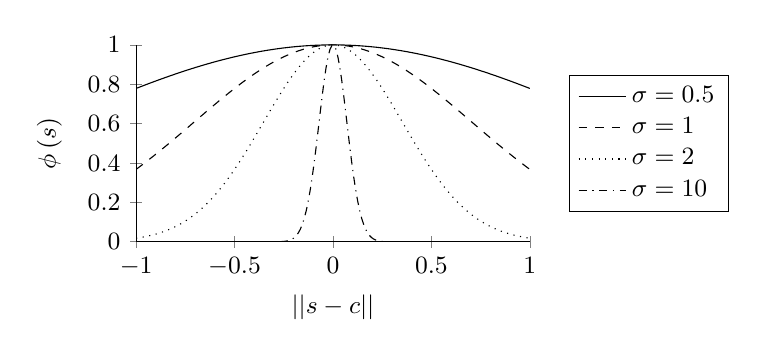
\begin{tikzpicture}
\begin{axis}[
    my cycle list, my axis, my scaling, my full width, my anchored legend, my samples,
    xlabel={$\left\lvert\left\lvert\state-\rbfcenter\right\rvert\right\rvert$},
    ylabel={$\featurevectorcomponent\left(\state\right)$},
    xmin=-1, xmax=1, ymin=0, ymax=1,
    domain=-1:1,
]
    \addplot+ {e^(-(0.5 * x)^2)};
    \addlegendentry{\small{$\rbfwidth=0.5$}};

    \addplot+ {e^(-(1 * x)^2)};
    \addlegendentry{\small{$\rbfwidth=1$}};

    \addplot+ {e^(-(2 * x)^2)};
    \addlegendentry{\small{$\rbfwidth=2$}};

    \addplot+ {e^(-(10 * x)^2)};
    \addlegendentry{\small{$\rbfwidth=10$}};
\end{axis}
\end{tikzpicture}

\caption{Response for various choices of~${\rbfwidth}$.}
\label{fig:rbf_by_width}
\end{figure}
As we will see later, such features require manual tuning in order to learn efficiently. Because of this, if possible, it is generally advisable to construct problem-specific features.

\subsection{Prediction with function approximation}
Update rule~\eqref{eq:vfa_sgd} cannot be performed. In fact, we do not have the true value function,~${\statevalue\policyscript\left(\state\right)}$, but we can substitute it with some approximation. For MC methods, the target is the return,~${\return_{\timestep}}$. For TD(0), the target is the TD target. For TD(${\lambda}$), the target is the~${\lambda}$-return,~${\return_{\timestep}^{\lambda}}$. We will see how prediction can be performed only in the last two cases, since MC methods do not extend as well to value function approximation.

Assuming linear value function approximation, the update rule for TD(0) becomes
\begin{align}
	\valueparameter
		&\gets\valueparameter-\gradientstep\left(\randomreward_{\timestep+1}+\discount\approximatestatevalue\left(\randomstate_{\timestep+1};\valueparameter\right)-\approximatestatevalue\left(\randomstate_{\timestep};\valueparameter\right)\right)\nabla_{\valueparameter}\approximatestatevalue\left(\randomstate_{\timestep};\valueparameter\right) \notag \\
		&=\valueparameter-\gradientstep\tderror_{\timestep}\featurevector\left(\randomstate_{\timestep}\right).
\end{align}
Instead, in the case of backward TD(${\lambda}$), we have,
\begin{align}
	\valueparameter
		&\gets\valueparameter-\gradientstep\left(\return_{\timestep}^{\lambda}-\approximatestatevalue\left(\randomstate_{\timestep};\valueparameter\right)\right)\nabla_{\valueparameter}\approximatestatevalue\left(\randomstate_{\timestep};\valueparameter\right) \notag \\
		&=\valueparameter-\gradientstep\left(\return_{\timestep}^{\lambda}-\approximatestatevalue\left(\randomstate_{\timestep};\valueparameter\right)\right)\featurevector\left(\randomstate_{\timestep}\right),
\end{align}
and in the case of forward TD(${\lambda}$)~\cite{sutton1988td},
\begin{equation}
\begin{split}
	\tderror_{\timestep}&=\randomreward_{\timestep+1}+\discount\approximatestatevalue\left(\randomstate_{\timestep+1};\valueparameter\right)-\approximatestatevalue\left(\randomstate_{\timestep};\valueparameter\right) \\
	\trace_{\timestep}&=\discount\lambda\trace_{\timestep-1}+\nabla_{\valueparameter}\approximatestatevalue\left(\randomstate_{\timestep};\valueparameter\right)=\discount\lambda\trace_{\timestep-1}+\featurevector\left(\randomstate_{\timestep}\right) \\
	\valueparameter&\gets\valueparameter-\gradientstep\tderror_{\timestep}\trace_{\timestep}.
\end{split}
\end{equation}

Unfortunately, however, in the case of linear value function approximation, we do not have the same convergence guarantees that we have in the tabular case. In fact, TD prediction has an asymptotic error which depends on the discount factor~${\discount}$~\cite{tsitsiklis1996}.

\subsection{Control with function approximation}
Recall that to do control in the model-free case we need to use the action-value function instead of the state-value function. This implies that rather than representing a state by a feature vector, we will now represent a state-action pair, as follows:
\begin{equation}
	\featurevector\left(\state,\action\right)\doteq\left(\featurevectorcomponent_{1}\left(\state,\action\right),\dots,\featurevectorcomponent_{\parametersize}\left(\state,\action\right)\right)^{\top}.
\end{equation}
This also causes the vector~${\valueparameter}$ to be of length~${\parametersize\cdot\left\lvert\actionspace\right\rvert}$. We can see this as having a (state-value) feature vector for each of the possible actions. In the linear case, a simple idea is that of appending the feature vector~${\lvert\actionspace\rvert}$ times and then set to zero the feature values of all actions except the currently selected one~\cite{lagoudakis2003lspi}, as follows:
\begin{equation}
	\featurevector\left(\state,\action\right)\doteq
	\begin{pmatrix}
		\featurevector\left(\state\right)\cdot\mathbf{1}\left(\randomaction_{\timestep}=\action_{1}\right) \\
		\vdots \\
		\featurevector\left(\state\right)\cdot\mathbf{1}\left(\randomaction_{\timestep}=\action_{\left\lvert\actionspace\right\rvert}\right)
	\end{pmatrix},
\end{equation}
and then updating the whole weight vector by stochastic gradient descent,
\begin{equation}
	\valueparameter\gets\valueparameter+\gradientstep\tderror_{\timestep}\featurevector\left(\randomstate_{\timestep},\randomaction_{\timestep}\right).
\end{equation}
Of course, copying the features many times is computationally very expensive. A better alternative is to leverage the sparsity of the vector and update only the relevant action. To do so, we reshape the value vector~$\valueparameter$ into a matrix of size~$\parametersize\times\left\lvert\actionspace\right\rvert$, and then update only the column corresponding to the selected action,
\begin{equation}
	\valueparameter_{\indexletter,\action}\gets\valueparameter_{\indexletter,\action}+\gradientstep\tderror_{\timestep}\featurevector\left(\randomstate_{\timestep}\right)~\textnormal{for}~\indexletter\in\left\{1,\dots,\parametersize\right\}~\textnormal{and}~\action=\randomaction_{\timestep}.
\end{equation}

Once again, in order to do control we apply the concept of generalized policy iteration, by interleaving (approximate) policy evaluation steps and policy improvement steps. However, in the linear case, SARSA ends up wandering around a bounded region near the optimal solution~\cite{gordon1996, gordon2001}, whereas Q-learning can even exhibit instability~\cite{baird1995}. Additionally, when doing control with nonlinear function approximators no theoretical guarantees have been proven.

\chapter{Policy-based reinforcement learning} \label{ch:policy_based_rl}
We will now introduce policy-based methods. Up to now, we presented only reinforcement learning methods that learned an action-value function, from which the target policy was implicitly derived. Policy-based methods directly optimize a stochastic policy instead.

The policy is generally modeled with a parameterized function with respect to a weight vector~${\policyparameter}$, and is denoted~${\policy_{\policyparameter}\left(\action\middle\vert\state\right)}$. The goal is to find~${\policyparameter}$ that maximizes an objective function~${\objective\left(\policyparameter\right)}$. Policy-based reinforcement learning is an optimization problem. We will focus on gradient methods, even though many other approaches can be used.

\section{Policy gradient}
Policy gradient methods search for a local maximum in~${\objective\left(\policyparameter\right)}$ by ascending the gradient of the policy, with respect to the parameter vector~${\policyparameter}$,
\begin{equation}
	\policyparameter\gets\policyparameter+\gradientstep\nabla_{\policyparameter}\objective\left(\policyparameter\right),
\end{equation}
where~${\gradientstep}$ is a step size parameter. We will also assume the sequence of step sizes~${\left\{\gradientstep_{\indexletter}\right\}}$ to be a Robbins-Monro sequence, as in~\eqref{eq:robbins_monro}. The gradient~${\nabla_{\policyparameter}\objective\left(\policyparameter\right)}$ is called the policy gradient, and is defined as
\begin{equation}
	\nabla_{\policyparameter}\objective\left(\policyparameter\right)\doteq\left(\frac{\partial\objective\left(\policyparameter\right)}{\partial\policyparametercomponent_{1}},\dots,\frac{\partial\objective\left(\policyparameter\right)}{\partial\policyparametercomponent_{\parametersize}}\right)^{\top}.
\end{equation}

\subsection{Analytic computation}
We will consider the simple case in which the MDP is episodic and~${\discount=1}$, although the following results can be extended to non-episodic MDPs and~${\discount<1}$. Let the objective function~${\objective\left(\policyparameter\right)}$ be the expected rewards for an episode,
\begin{align}
	\objective\left(\policyparameter\right)
		&\doteq\mathbb{E}_{\left(\randomstate_{\timestep},\randomaction_{\timestep}\right)\sim\policy_{\policyparameter}}\left[\sum_{\timestep=1}^{\horizon}\randomreward_{\timestep}\right] \notag \\
		&=\mathbb{E}_{\trajectory\sim\policy_{\policyparameter}}\left[\immediatereward\left(\trajectory\right)\right] \notag \\
		&=\sum_{\trajectory}\transition_{\policyparameter}\left(\trajectory\right)\immediatereward\left(\trajectory\right),	
\end{align}
where~${\trajectory}$ is a trajectory,~${\left(\randomstate_{0},\randomaction_{0},\randomreward_{1},\randomstate_{1},\randomaction_{1},\randomreward_{2},\dots,\randomstate_{\horizon-1},\randomaction_{\horizon-1},\randomreward_{\horizon}\right)}$,~${\transition_{\policyparameter}\left(\trajectory\right)}$ denotes the probability of sampling a trajectory~${\trajectory}$ when following policy~${\policy_{\policyparameter}}$, i.e.,~${\trajectory\sim\transition_{\policyparameter}\left(\trajectory\right)}$, and~${\immediatereward\left(\trajectory\right)}$ is the sum of rewards for a trajectory~${\trajectory}$.

Assuming that we can compute the policy gradient~${\nabla_{\policyparameter}\policy_{\policyparameter}\left(\action\middle\vert\state\right)}$, then we can compute the policy gradient, as follows:
\begin{align} \label{eq:obj_function_derivative}
	\nabla_{\policyparameter}\objective\left(\policyparameter\right)
		&=\nabla_{\policyparameter}\sum_{\trajectory}\transition_{\policyparameter}\left(\trajectory\right)\immediatereward\left(\trajectory\right) \notag \\
		&=\sum_{\trajectory}\nabla_{\policyparameter}\transition_{\policyparameter}\left(\trajectory\right)\immediatereward\left(\trajectory\right) \notag \\
		&=\sum_{\trajectory}\frac{\transition_{\policyparameter}\left(\trajectory\right)}{\transition_{\policyparameter}\left(\trajectory\right)}\nabla_{\policyparameter}\transition_{\policyparameter}\left(\trajectory\right)\immediatereward\left(\trajectory\right) \notag \\
		&=\sum_{\trajectory}\transition_{\policyparameter}\left(\trajectory\right)\immediatereward\left(\trajectory\right)\frac{\nabla_{\policyparameter}\transition_{\policyparameter}\left(\trajectory\right)}{\transition_{\policyparameter}\left(\trajectory\right)} \notag \\
		&=\sum_{\trajectory}\transition_{\policyparameter}\left(\trajectory\right)\immediatereward\left(\trajectory\right)\nabla_{\policyparameter}\log\transition_{\policyparameter}\left(\trajectory\right) \notag \\
		&=\mathbb{E}_{\trajectory\sim\policy_{\policyparameter}}\left[\immediatereward\left(\trajectory\right)\nabla_{\policyparameter}\log\transition_{\policyparameter}\left(\trajectory\right)\right],
\end{align}
where the second to last equality follows from~${\nabla\log{f\left(x\right)}=\frac{\nabla{f\left(x\right)}}{f\left(x\right)}}$ which, in turn, follows by the chain rule. This is also known as the REINFORCE trick~\cite{williams1992reinforce}.

Since the expectation~${\mathbb{E}_{\trajectory\sim\policy_{\policyparameter}}\left[\cdot\right]}$ can be estimated by sample averages, we only need the derivative~${\nabla_{\policyparameter}\log\transition_{\policyparameter}\left(\trajectory\right)}$. Importantly, this derivative can be computed without knowledge of the initial state distribution, or the dynamics of the MDP. In fact, we have that
\begin{align} \label{eq:log_derivative_trick}
	\nabla_{\policyparameter}\log\transition_{\policyparameter}\left(\trajectory\right)
		&=\nabla_{\policyparameter}\log\left(\initialdistribution\left(\randomstate_{0}\right)\prod_{\timestep=0}^{\horizon-1}\transition\left(\randomstate_{\timestep+1}\middle\vert\randomstate_{\timestep},\randomaction_{\timestep}\right)\policy_{\policyparameter}\left(\randomaction_{\timestep}\middle\vert\randomstate_{\timestep}\right)\right) \notag \\
		&\overset{(a)}{=}\nabla_{\policyparameter}\left(\log\initialdistribution\left(\randomstate_{0}\right)+\sum_{\timestep=0}^{\horizon-1}\log\transition\left(\randomstate_{\timestep+1}\middle\vert\randomstate_{\timestep},\randomaction_{\timestep}\right)+\sum_{\timestep=0}^{\horizon-1}\log\policy_{\policyparameter}\left(\randomaction_{\timestep}\middle\vert\randomstate_{\timestep}\right)\right) \notag \\
		&\overset{(b)}{=}\sum_{\timestep=0}^{\horizon-1}\nabla_{\policyparameter}\log\policy_{\policyparameter}\left(\randomaction_{\timestep}\middle\vert\randomstate_{\timestep}\right),
\end{align}
where
\begin{enumerate*}[label=(\alph*)]
	\item follows from~${\log\left(ab\right)=\log{a}+\log{b}}$, and
	\item follows from the fact that only the policy depends on~${\policyparameter}$.
\end{enumerate*}
The gradient~${\nabla_{\policyparameter}\log\policy_{\policyparameter}\left(\action\middle\vert\state\right)}$ is known as the score function. Thus, by combining~\eqref{eq:obj_function_derivative} and~\eqref{eq:log_derivative_trick}, we have that
\begin{equation}
	\nabla_{\policyparameter}\objective\left(\policyparameter\right)=\mathbb{E}_{\trajectory\sim\policy_{\policyparameter}}\left[\immediatereward\left(\trajectory\right)\sum_{\timestep=0}^{\horizon-1}\nabla_{\policyparameter}\log\policy_{\policyparameter}\left(\randomaction_{\timestep}\middle\vert\randomstate_{\timestep}\right)\right].
\end{equation}

\subsection{Policy gradient theorem}
A more general theorem, known as the policy gradient theorem~\cite{marbach2001, sutton2000}, allows us to substitute the sum of rewards in a trajectory,~${\immediatereward\left(\trajectory\right)}$, with the action-value function,~${\actionvalue\policyscript\left(\state,\action\right)}$. Formally, the policy gradient, becomes
\begin{equation} \label{eq:policy_gradient_theorem}
	\nabla_{\policyparameter}\objective\left(\policyparameter\right)=\mathbb{E}_{\policy_{\policyparameter}}\left[\sum_{\timestep=0}^{\infty}\actionvalue\script{\policy_{\policyparameter}}\left(\randomstate_{\timestep},\randomaction_{\timestep}\right)\nabla_{\policyparameter}\log\policy_{\policyparameter}\left(\randomaction_{\timestep}\middle\vert\randomstate_{\timestep}\right)\right].
\end{equation}
This update has no bias but high variance. Many variants have been proposed in order to reduce the variance while keeping the bias unchanged~\cite{schulman2015gae}. In general, they take the form
\begin{equation}
	\nabla_{\policyparameter}\objective\left(\policyparameter\right)=\mathbb{E}_{\policy_{\policyparameter}}\left[\sum_{\timestep=0}^{\infty}\Psi_{\timestep}\nabla_{\policyparameter}\log\policy_{\policyparameter}\left(\randomaction_{\timestep}\middle\vert\randomstate_{\timestep}\right)\right].
\end{equation}
We will see the cases in which~${\Psi_{\timestep}}$ is the return starting at time step~${\timestep}$,~${\return_{\timestep}}$, and the TD target,~${\randomreward_{\timestep+1}+\discount\estimatestatevalue\left(\randomstate_{\timestep+1}\right)}$.

\section{Differentiable policies}
Prior to introducing any policy gradient method, we will see two kinds of policies commonly used that are differentiable with respect to the parameter vector~${\policyparameter}$.

\subsection{Softmax policy}
If the action space is discrete and not too large, the softmax function is generally used to parameterize the policy. It is defined as:
\begin{equation} \label{eq:softmax_policy}
	\policy_{\policyparameter}\left(\action\middle\vert\state\right)\doteq\frac{e^{\featurevector\left(\state,\action\right)^{\top}\policyparameter}}{\sum_{\varaction}e^{\featurevector\left(\state,\varaction\right)^{\top}\policyparameter}}.
\end{equation}
The score function can be derived as follows:
\begin{align} \textbf{\label{eq:softmax_part1}}
	\nabla_{\policyparameter}\log\policy_{\policyparameter}\left(\action\middle\vert\state\right)
		&=\nabla_{\policyparameter}\log\frac{e^{\featurevector\left(\state,\action\right)^{\top}\policyparameter}}{\sum_{\varaction}e^{\featurevector\left(\state,\varaction\right)^{\top}\policyparameter}} \notag \\
		&=\nabla_{\policyparameter}\log{e^{\featurevector\left(\state,\action\right)^{\top}}\policyparameter}-\nabla_{\policyparameter}\log\sum_{\varaction}e^{\featurevector\left(\state,\varaction\right)^{\top}\policyparameter},
\end{align}
where the equality follows from~${\log\frac{a}{b}=\log{a}-\log{b}}$. The first term can be derived easily,
\begin{equation}
	\nabla_{\policyparameter}\log{e^{\featurevector\left(\state,\action\right)^{\top}}\policyparameter}=\nabla_{\policyparameter}\featurevector\left(\state,\action\right)^{\top}\policyparameter=\featurevector\left(\state,\action\right),
\end{equation}
while the second one requires a bit more work,
\begin{align}
	\nabla_{\policyparameter}\log\sum_{\varaction}e^{\featurevector\left(\state,\varaction\right)^{\top}\policyparameter}
		&\overset{(a)}{=}\frac{\nabla_{\policyparameter}\sum_{\varaction}e^{\featurevector\left(\state,\varaction\right)^{\top}\policyparameter}}{\sum_{\varaction}e^{\featurevector\left(\state,\varaction\right)^{\top}\policyparameter}} \notag \\
		&\overset{(b)}{=}\frac{\sum_{\varaction}\featurevector\left(\state,\varaction\right)e^{\featurevector\left(\state,\varaction\right)^{\top}\policyparameter}}{\sum_{\varaction}e^{\featurevector\left(\state,\varaction\right)^{\top}\policyparameter}} \notag \\
		&\overset{(c)}{=}\sum_{\varaction}\featurevector\left(\state,\varaction\right)\policy_{\policyparameter}\left(\varaction\middle\vert\state\right) \notag \\
		&=\mathbb{E}_{\policy_{\policyparameter}}\left[\featurevector\left(\state,\cdot\right)\right],
\end{align}
where
\begin{enumerate*}[label=(\alph*)]
	\item follows by the chain rule,
	\item follows again by the chain rule, and
	\item follows by the definition of~${\policy_{\policyparameter}}$~\eqref{eq:softmax_policy}.
\end{enumerate*}
Putting everything together, we have that the score function is
\begin{equation} \label{eq:softmax_score}
	\nabla_{\policyparameter}\log\policy_{\policyparameter}\left(\action\middle\vert\state\right)=\featurevector\left(\state,\action\right)-\mathbb{E}_{\policy_{\policyparameter}}\left[\featurevector\left(\state,\cdot\right)\right].
\end{equation}

\subsection{Gaussian policy}
A typical choice in the case of continuous actions spaces is a Gaussian policy~\cite{williams1992reinforce}. Both the mean and the variance can be parameterized (in which case the parameter vector would be~${\policyparameter=\left(\policyparameter_{\mu},\policyparameter_{\sigma}\right)^{\top}}$), but we will assume for the variance to be fixed.

Actions are sampled from a normal probability distribution,~${\action\sim\mathcal{N}\left(\mu_{\policyparameter}\left(\state\right),\sigma^{2}\right)}$, that is
\begin{equation}
	\policy_{\policyparameter}\left(\action\middle\vert\state\right)\doteq\frac{1}{\sigma\sqrt{2\pi}}\exp\left(-\frac{\left(\action-\mu_{\policyparameter}\left(\state\right)\right)^{2}}{2\sigma^{2}}\right),
\end{equation}
where the mean is a linear combination of state features,~${\mu_{\policyparameter}\left(\state\right)=\featurevector\left(\state\right)^{\top}\policyparameter}$. Thus, the score function is:
\begin{align}
	\nabla_{\policyparameter}\log\policy_{\policyparameter}\left(\action\middle\vert\state\right)
		&\overset{(a)}{=}\nabla_{\policyparameter}\log\exp\left(-\frac{\left(\action-\mu_{\policyparameter}\left(\state\right)\right)^{2}}{2\sigma^{2}}\right)-\nabla_{\policyparameter}\log\frac{1}{\sigma\sqrt{2\pi}} \notag \\
		&\overset{(b)}{=}-\frac{1}{2\sigma^{2}}\nabla_{\policyparameter}\left(\action-\mu_{\policyparameter}\left(\state\right)\right)^{2} \notag \\
		&\overset{(c)}{=}-\frac{1}{2\sigma^{2}}\left(-2\left(\action-\mu_{\policyparameter}\left(\state\right)\right)\nabla_{\policyparameter}\mu_{\policyparameter}\left(\state\right)\right) \notag \\
		&\overset{(d)}{=}\frac{\left(\action-\mu_{\policyparameter}\left(\state\right)\right)\featurevector\left(\state\right)}{\sigma^2}.
\end{align}
where
\begin{enumerate*}[label=(\alph*)]
	\item follows from~${\log\frac{a}{b}=\log{a}-\log{b}}$,
	\item follows from the fact that the second term does not depend on~${\policyparameter}$,
	\item follows by the chain rule, and
	\item follows from~${\nabla_{\policyparameter}\mu_{\policyparameter}\left(\state\right)=\featurevector\left(\state\right)}$.
\end{enumerate*}

\section{Basic policy gradient algorithms}
We are now ready to introduce some basic policy gradient algorithms. First, we will see REINFORCE~\cite{williams1992reinforce}, which can be simply described as Monte Carlo policy gradient. Then, we will add a critic as a simple way to reduce the variance.

\subsection{REINFORCE}
The REINFORCE algorithm uses the return~${\return_{\timestep}}$ as an unbiased sample of~${\actionvalue\policyscript\left(\randomstate_{\timestep},\randomaction_{\timestep}\right)}$, as in value-based Monte Carlo. In particular, we will sample an episode following~${\policy_{\policyparameter}}$, then, for each time step~${\timestep}$ of the episode, we estimate the policy gradient~\eqref{eq:policy_gradient_theorem}, and update the parameter vector~${\policyparameter}$ according to stochastic gradient ascent,
\begin{equation} \label{eq:reinforce_update}
	\policyparameter\gets\policyparameter+\gradientstep\return_{\timestep}\nabla_{\policyparameter}\log\policy_{\policyparameter}\left(\randomaction_{\timestep}\middle\vert\randomstate_{\timestep}\right).
\end{equation}
The pseudo-code for the REINFORCE algorithm is given in Algorithm~\ref{alg:reinforce}.
\begin{algorithm}
	\caption{REINFORCE, estimating~${\policy_{\policyparameter}\approx\policy\optimal}$}
	\label{alg:reinforce}

	\Function{$\textup{\textsc{REINFORCE}}\left(\gradientstep\right)$}{
		$\policyparameter_{\indexletter}\gets0$, for $\indexletter\in\left\{1,\dots,\parametersize\right\}$\;
		\Loop{}{
			Sample an episode following $\policy_{\policyparameter}$: $\left(\randomstate_{0},\randomaction_{0},\randomreward_{1},\dots,\randomstate_{\horizon-1},\randomaction_{\horizon-1},\randomreward_{\horizon}\right)$\;
			\ForEach{$\left(\randomstate_{\timestep},\randomaction_{\timestep}\right)$}{
				$\return_{\timestep}\gets\sum_{\indexletter=\timestep+1}^{\horizon}\discount^{\indexletter-\timestep-1}\randomreward_{\indexletter}$\;
				$\policyparameter\gets\policyparameter+\gradientstep\return_{\timestep}\nabla\log\policy_{\policyparameter}\left(\randomaction_{\timestep}\middle\vert\randomstate_{\timestep}\right)$\;
			}
		}
		\KwRet{$\policy_{\policyparameter}$}\;
	}
\end{algorithm}

Of course, as a Monte Carlo method, REINFORCE has high variance. A common way to reduce variance is to introduce a baseline,~${\baseline\left(\state\right)}$, into the expectation. The baseline can be any function, as long as it does not vary with~${\action}$. The gradient now takes the form
\begin{equation}
	\nabla_{\policyparameter}\objective\left(\policyparameter\right)=\mathbb{E}_{\policy_{\policyparameter}}\left[\sum_{\timestep=0}^{\horizon-1}\left(\return_{\timestep}-\baseline\left(\randomstate_{\timestep}\right)\right)\nabla_{\policyparameter}\log\policy_{\policyparameter}\left(\randomaction_{\timestep}\middle\vert\randomstate_{\timestep}\right)\right].
\end{equation}
This can be done as subtracting a baseline is unbiased in expectation, in fact we have that
\begin{align}
	\mathbb{E}_{\policy_{\policyparameter}}\left[\nabla_{\policyparameter}\log\transition_{\policyparameter}\left(\trajectory\right)\baseline\right]
		&=\sum_{\trajectory}\transition_{\policyparameter}\left(\trajectory\right)\nabla_{\policyparameter}\log\transition_{\policyparameter}\left(\trajectory\right)\baseline \notag \\
		&=\sum_{\trajectory}\nabla_{\policyparameter}\transition_{\policyparameter}\left(\trajectory\right)\baseline \notag \\
		&=\baseline\nabla_{\policyparameter}\sum_{\trajectory}\transition_{\policyparameter}\left(\trajectory\right) \notag \\
		&=\baseline\nabla_{\policyparameter}1=0.
\end{align}

A typical choice for the baseline is the state-value function,~${\baseline\left(\state\right)=\statevalue\policyscript\left(\state\right)}$. This allows us to rewrite the policy gradient using the so-called advantage function,~${\advantage\policyscript}$,
\begin{equation}
\begin{split}
	\advantage\policyscript\left(\state,\action\right)&\doteq\actionvalue\policyscript\left(\state,\action\right)-\statevalue\policyscript\left(\state\right) \\
	\nabla_{\policyparameter}\objective\left(\policyparameter\right)&=\mathbb{E}_{\policy_{\policyparameter}}\left[\sum_{\timestep=0}^{\horizon-1}\advantage\policyscript\left(\randomstate_{\timestep},\randomaction_{\timestep}\right)\nabla_{\policyparameter}\log\policy_{\policyparameter}\left(\randomaction_{\timestep}\middle\vert\randomstate_{\timestep}\right)\right],
\end{split}
\end{equation}
since the return is an unbiased estimate of~${\actionvalue\policyscript\left(\randomstate_{\timestep},\randomaction_{\timestep}\right)}$. Intuitively, the advantage function measures how much better or worse it is to take action~${\action}$ in state~${\state}$, rather than randomly sampling an action according to~${\policy_{\policyparameter}\left(\cdot\middle\vert\state\right)}$. Algorithm~\ref{alg:reinforce} can be modified to use a baseline by simply replacing the return with the advantage function in the update step defined in~\eqref{eq:reinforce_update}, where the advantage function is approximated by~${\return_{\timestep}-\approximatestatevalue\left(\randomstate_{\timestep};\valueparameter\right)}$, for some weight vector~${\valueparameter}$.

\subsection{Actor-critic}
In actor-critic methods~\cite{barto1983} we have a critic, which estimates the value function, and an actor, which updates the policy in the direction suggested by the critic.

The REINFORCE algorithm with a baseline can indeed be seen as a case of actor-critic. In fact, in the case presented the baseline is an estimate of the state-value function. Alternatively, we can reduce variance and accelerate learning by using bootstrapping methods for prediction, such as the ones introduced in sections~\ref{sec:td_prediction} and~\ref{sec:td_lambda}. Of course, this is done at the cost of introducing some bias, since bootstrapping methods update their estimate based on the current estimate of subsequent states. We will only see the case for TD(0), as generalizing the concepts to TD(${\lambda}$) is straightforward. In this case the algorithm is called one-step actor-critic. We replace the full return,~${\return_{\timestep}}$, with the TD target in the gradient update, as follows:
\begin{align}
	\policyparameter
		&\gets\policyparameter+\gradientstep\left(\return_{\timestep}-\approximatestatevalue\left(\randomstate_{\timestep};\valueparameter\right)\right)\nabla_{\policyparameter}\log\policy_{\policyparameter}\left(\randomaction_{\timestep}\middle\vert\randomstate_{\timestep}\right) \notag \\
		&=\policyparameter+\gradientstep\left(\randomreward_{\timestep+1}+\discount\approximatestatevalue\left(\randomstate_{\timestep+1};\valueparameter\right)-\approximatestatevalue\left(\randomstate_{\timestep};\valueparameter\right)\right)\nabla_{\policyparameter}\log\policy_{\policyparameter}\left(\randomaction_{\timestep}\middle\vert\randomstate_{\timestep}\right) \notag \\
		&=\policyparameter+\gradientstep\tderror_{\timestep}\nabla_{\policyparameter}\log\policy_{\policyparameter}\left(\randomaction_{\timestep}\middle\vert\randomstate_{\timestep}\right)
\end{align}
Algorithm~\ref{alg:actor_critic} shows the pseudo-code for the one-step actor-critic algorithm.
\begin{algorithm}
	\caption{One step actor-critic, estimating~${\policy_{\policyparameter}\approx\policy\optimal}$}
	\label{alg:actor_critic}

	\Function{$\textup{\textsc{OneStepActorCritic}}\left(\gradientstep_{\policyparameter},\gradientstep_{\valueparameter}\right)$}{
		$\policyparameter_{\indexletter}\gets0$, for $\indexletter\in\left\{1,\dots,\parametersize_{\policyparameter}\right\}$\;
		$\valueparameter_{\indexletter}\gets 0$, for $\indexletter\in\left\{1,\dots,\parametersize_{\valueparameter}\right\}$\;
		\Loop{}{
			$\randomstate_{0}\sim\initialdistribution\left(\cdot\right)$\;
			\Loop{\textup{for each step of the episode}}{
				$\randomaction_{\timestep}\sim\policy_{\policyparameter}\left(\cdot\middle\vert\randomstate_{\timestep}\right)$\;
				$\randomstate_{\timestep+1}\sim\transition\left(\cdot\middle\vert\randomstate_{\timestep},\randomaction_{\timestep}\right)$, $\randomreward_{\timestep+1}\gets\immediatereward\left(\randomstate_{\timestep},\randomaction_{\timestep}\right)$\;
				$\tderror_{\timestep}\gets\randomreward_{\timestep+1}+\discount\approximatestatevalue\left(\randomstate_{\timestep+1},\randomaction_{\timestep+1};\valueparameter\right)-\approximatestatevalue\left(\randomstate_{\timestep},\randomaction_{\timestep};\valueparameter\right)$\;
				$\policyparameter\gets\policyparameter+\gradientstep_{\policyparameter}\tderror_{\timestep}\nabla_{\policyparameter}\log\policy_{\policyparameter}\left(\randomaction_{\timestep}\middle\vert\randomstate_{\timestep}\right)$\;
				$\valueparameter\gets\valueparameter-\gradientstep_{\valueparameter}\tderror_{\timestep}\featurevector\left(\randomstate_{\timestep},\randomaction_{\timestep}\right)$\;
				$\randomstate_{\timestep}\gets\randomstate_{\timestep+1}$\;
			}
		}
		\KwRet{$\policy_{\policyparameter}$}\;
	}
\end{algorithm}

\subsection{Comparison of value- and policy-based methods}
Policy-based methods were the earliest to be studied in reinforcement learning, but they were neglected in favor of value-based methods starting from the introduction of Q-learning~\cite{watkins1989learning}. In recent years, however, several developments~\cite{peters2008, degris2012, silver2014} have shifted once again the focus on policy-gradient methods.

Although policy-gradient methods generally converge locally, they still have better convergence properties than value-based methods with function approximation. Additionally, they can learn stochastic policies, which are beneficial in the case of games, since repetitive actions can be exploited by the opponents, and environments in which the observations of the state are not fully representative, as in this case some states share the same observation, thus possibly causing deterministic policies to always choose non-optimal actions. Ultimately, as we have seen, they can even be employed with both high-dimensional and continuous action spaces.

\chapter{Empirical results} \label{ch:empirical_results}
We now move on from theory by running some experiments using the methods presented in the previous chapters. We start by presenting the environments used, then, just as in the first part, we will first present results in the case in which both the state and the action space are finite, and then the case in which the state space is continuous.

\section{Domains}
In this section we present the environments on which we will run the experiments. The first two environments have a finite state space, while the third one has a continuous state space. Additionally, in the third environment we have the possibility of either choosing the variant with a finite action space, or the variant with a continuous action space.

\subsection{Cliff walking}
The cliff walking environment~\cite[Example 6.6]{suttonbarto1998reinforcementlearning} is a~${4\times12}$ grid in which the agent has to travel from a starting point~{(S)} to a goal~{(G)}, as shown in Figure~\ref{fig:cliff_walking}. At each time step the agent receives a reward of~{-1}, and a reward of~{-100} if it falls into the cliff, which resets the agent back to the starting point. The goal is a terminal state, meaning that any action taken in that state will transition to itself, with reward 0.
\begin{figure}
\centering
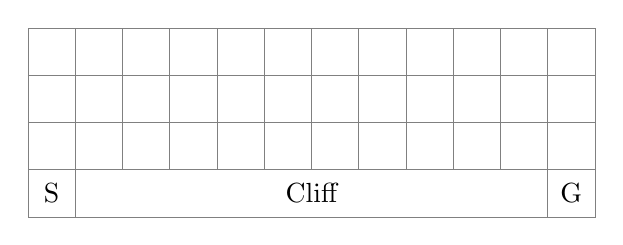
\begin{tikzpicture}[scale=0.60]
    \draw[gray,very thin] ( 0, 1) --
                          ( 0, 0) --
                          ( 1, 0) --
                          ( 1, 1);
    \draw[gray,very thin] ( 1, 0) -- (11, 0);
    \draw[gray,very thin] (11, 1) --
                          (11, 0) --
                          (12, 0) --
                          (12, 1);
    \draw[step=1cm,gray,very thin] (0, 1) grid (12, 4);
    \draw (0.5, 0.5) node {S};
    \draw (11.5, 0.5) node {G};
    \draw (6, 0.5) node {Cliff};
\end{tikzpicture}

\caption{Cliff walking environment.}
\label{fig:cliff_walking}
\end{figure}

Since the agent receives a reward of -1 for each time step, it is incentivized to reach the goal as fast as possible. Clearly, this implies that the optimal policy is the one that walks closest to the cliff, obtaining a cumulative reward of -13 for each episode.

\subsection{Frozen lake}
The frozen lake environment is a~${4\times4}$ grid in which the agent has to cross the frozen lake from a starting point~{(S)} to a goal~{(G)} while avoiding holes~{(H)}. The default configuration of the grid and the according optimal policy are shown in Figure~\ref{fig:frozen_lake}. Due to the slippery nature of the lake, the agent will move towards its intended direction with probability~${1/3}$, else it will move in either of the perpendicular directions with an equal probability of~${1/3}$. The reward is 1 if the agent reaches the goal, and 0 otherwise.
\begin{figure}
\centering
\begin{subfigure}{0.3\textwidth}
	\centering
	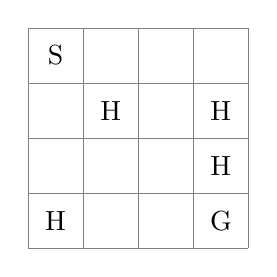
\begin{tikzpicture}[scale=0.7]
    \draw[step=1cm,gray,very thin] (0, 0) grid (4, 4);
    \draw (0.5, 3.5) node {S};
    \draw (0.5, 0.5) node {H};
    \draw (1.5, 2.5) node {H};
    \draw (3.5, 2.5) node {H};
    \draw (3.5, 1.5) node {H};
    \draw (3.5, 0.5) node {G};
\end{tikzpicture}

	\caption{Environment.}
\end{subfigure}
\begin{subfigure}{0.3\textwidth}
	\centering
	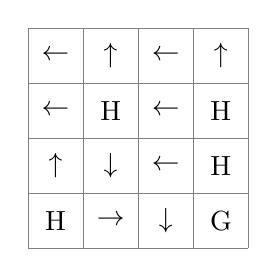
\begin{tikzpicture}[scale=0.7]
    \draw[step=1cm,gray,very thin] (0, 0) grid (4, 4);
    \draw (0.5, 3.5) node {$\leftarrow$};
    \draw (1.5, 3.5) node {$\uparrow$};
    \draw (2.5, 3.5) node {$\leftarrow$};
    \draw (3.5, 3.5) node {$\uparrow$};
    \draw (0.5, 2.5) node {$\leftarrow$};
    \draw (1.5, 2.5) node {H};
    \draw (2.5, 2.5) node {$\leftarrow$};
    \draw (3.5, 2.5) node {H};
    \draw (0.5, 1.5) node {$\uparrow$};
    \draw (1.5, 1.5) node {$\downarrow$};
    \draw (2.5, 1.5) node {$\leftarrow$};
    \draw (3.5, 1.5) node {H};
    \draw (0.5, 0.5) node {H};
    \draw (1.5, 0.5) node {$\rightarrow$};
    \draw (2.5, 0.5) node {$\downarrow$};
    \draw (3.5, 0.5) node {G};
\end{tikzpicture}

	\caption{Optimal policy.}
\end{subfigure}
\caption{Frozen lake environment.}
\label{fig:frozen_lake}
\end{figure}

Intuitively, the solution can be explained as follows: the best policy is to move in such a way that both the intended direction, as well as its perpendicular directions, do not result in falling into a hole. Thus, here the objective is to reach the goal as safely as possible, rather than as fast as possible.

\subsection{Mountain car}
In the mountain car environment~\cite{moore1990control} a car placed at the bottom of a valley has to reach a goal state on top of a hill. Due to the steepness of the valley, the car cannot simply accelerate forwards and reach the goal. Instead, it has to sway from one hill to the other until it has gained enough momentum to get to the top. Figure~\ref{fig:mountain_car} is a visual representation of the environment.
\begin{figure}
\centering
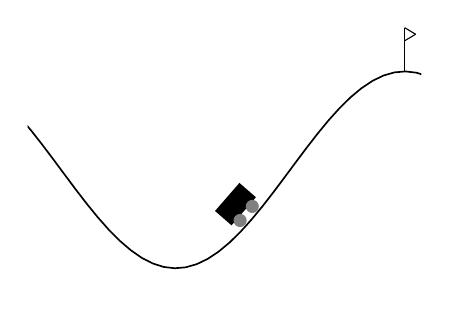
\begin{tikzpicture}
\begin{axis}[
    my full width, my samples,
    xmin=-1.2, xmax=0.6, ymin=0, ymax=1.2,
    x axis line style={draw=none},
    y axis line style={draw=none},
    xtick={\empty},
    ytick={\empty},
    scale only axis,
    axis equal image,
]
    % Hills
    \addplot+[semithick, draw=black, mark=none] {sin(deg(3 * x)) * 0.45 + 0.55};

    % Goal flag
    \draw (pi / 6, 1) -- (pi / 6, 1.2);
    \draw (pi / 6, 1.2) -- (pi / 6 + 0.05, 1.17);
    \draw (pi / 6 + 0.05, 1.17) -- (pi / 6, 1.14);

    % Car
    \pgfmathsetmacro{\carrotataion}{49}
    \pgfmathsetmacro{\carwidth}{0.17};
    \pgfmathsetmacro{\carheight}{0.1};
    \pgfmathsetmacro{\carposx}{-0.25};
    \pgfmathsetmacro{\carposy}{sin(deg(3 * \carposx)) * 0.45 + 0.55 + \carheight / 2 + 0.1};
    \draw[
        % rotate around={cos(deg(3 * \carposx)):(\carposx, \carposy)}
        rotate around={\carrotataion:(\carposx, \carposy)},
        draw=none,
        fill=black
    ]
        (\carposx - \carwidth / 2, \carposy - \carheight / 2) rectangle
        (\carposx + \carwidth / 2, \carposy + \carheight / 2);

    % Wheels
    \pgfmathsetmacro{\wheelradius}{0.03};
    \draw[
        rotate around={\carrotataion:(\carposx, \carposy)},
        draw=none,
        fill=gray
    ]
        (\carposx - \carwidth / 4, \carposy - \carheight / 2 - \wheelradius / 2)
        circle [radius=\wheelradius];
    \pgfmathsetmacro{\wheelradius}{0.03};
    \draw[
        rotate around={\carrotataion:(\carposx, \carposy)},
        draw=none,
        fill=gray
    ]
        (\carposx + \carwidth / 4, \carposy - \carheight / 2 - \wheelradius / 2)
        circle [radius=\wheelradius];
\end{axis}
\end{tikzpicture}

\caption{Mountain car environment.}
\label{fig:mountain_car}
\end{figure}

The state is a tuple containing the position of the car along the x-axis and the velocity of the car. There are two variants of the environment, the first one has~3 discrete actions (accelerate to the left, do not accelerate, accelerate to the right), whereas the second one takes as an action a value between~${\left[-1,1\right]}$ representing the directional force applied to the car. Additionally, in the continuous action space case, the car is penalized for taking actions of large magnitude. In both cases the maximum number of steps per episode has been set to~10000.

\section{Finite state space experiments}
We will now compare the theoretical results presented in the first two chapters, with empirical results obtained in these environments. We will also observe that even in such simple problems, both the choice of the method to be used, as well as its parameters, is not straightforward. In order to assess how well the reinforcement learning agents have trained, we will use the mean squared error between the optimal value, computed via dynamic programming, and the estimate value.

\subsection{Policy and value iteration}
We first present an example comparing policy and value iteration. We will consider the cliff walking problem. Since the the environment has a terminal state, we can also consider the case in which~${\discount=1}$.

Figure~\ref{fig:pi_convergence} presents the maximum change in the value function for each full sweep of the state space, for the first prediction step of policy iteration, with different discount values.
\begin{figure}
\centering
\begin{tikzpicture}
\begin{axis}[
    my cycle list, my axis, my scaling, my full width, my anchored legend,
    xlabel=Full sweeps of the state space,
    ylabel=${\left\lvert\left\lvert\estimatestatevalue-\estimatestatevalue'\right\rvert\right\rvert_{\infty}}$,
    xmin=1, xmax=1e5, ymin=1e-3, ymax=250,
    xmode=log, ymode=log,
]
    \addplot+ table[x=sweep, y=delta] {tikz/data/policy_iteration_delta/0_9.dat};
    \addlegendentry{$\discount=0.9$};

    \addplot+ table[x=sweep, y=delta] {tikz/data/policy_iteration_delta/0_95.dat};
    \addlegendentry{$\discount=0.95$};

    \addplot+ table[x=sweep, y=delta] {tikz/data/policy_iteration_delta/0_99.dat};
    \addlegendentry{$\discount=0.99$};

    \addplot+ table[x=sweep, y=delta] {tikz/data/policy_iteration_delta/1.dat};
    \addlegendentry{$\discount=1$};
\end{axis}
\end{tikzpicture}

\caption{Convergence rate for the first prediction step of policy iteration.}
\label{fig:pi_convergence}
\end{figure}
The learned policy is the same for each of the optimal value functions obtained with the various discount factors, yet the number of sweeps needed for the first prediction step varies widely. Table~\ref{tab:policy_iteration_convergence} illustrates this.
\begin{table}
\centering
\begin{tabular}{l c c}
\toprule
${\discount}$ & Avg. number of sweeps & Iterations \\
\midrule
0.9 & 63 & 13 \\
0.95 & 127 & 12 \\
0.99 & 282 & 9 \\
1 & 4298 & 9 \\
\bottomrule
\end{tabular}
\caption{Average number of sweeps in the prediction step of policy iteration and total number of iterations needed to converge to the optimal policy.}
\label{tab:policy_iteration_convergence}
\end{table}
Furthermore, as the discount factor gets smaller, each of the prediction steps is less precise, thus requiring more iterations in order to converge to the optimal policy.

Interestingly, policy iteration still converges to the optimal value function with~${\discount=1}$ when stopping the prediction step to a maximum upper bound of sweeps of the state space (e.g.,~100), clearly indicating that convergence in the prediction step is not always necessary to converge to the optimal policy.

In this problem, value iteration simply requires one iteration to converge to the optimal value. Of course, the initial value function and policy influence significantly the convergence rate of both methods.

\subsection{Scheduling strategies for~\texorpdfstring{${\varepsilon}$}{epsilon}}
We now move onto reinforcement learning methods. We will start by comparing different scheduling strategies for~${\varepsilon}$ with various methods. In figure~\ref{fig:epsilon_schedules} the schedules taken into consideration are shown.
\begin{figure}[ht]
\centering
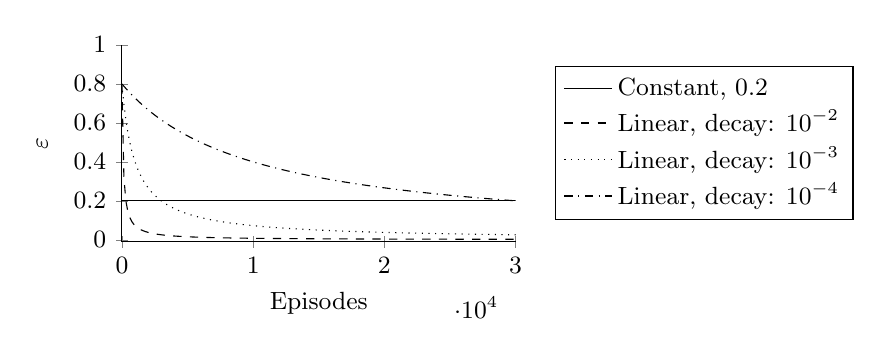
\begin{tikzpicture}
\begin{axis}[
    my cycle list, my axis, my scaling, my full width, my anchored legend, my samples,
    xlabel={Episodes},
    ylabel={$\varepsilon$},
    xmin=0, xmax=30000, ymin=-0.01, ymax=1,
    domain=1:30000,
]
    \addplot+ {0.2};
    \addlegendentry{\small{Constant, $0.2$}};

    \addplot+ {0.8/(1+(1e-2*x))};
    \addlegendentry{\small{Linear, decay: $10^{-2}$}};

    \addplot+ {0.8/(1+(1e-3*x))};
    \addlegendentry{\small{Linear, decay: $10^{-3}$}};

    \addplot+ {0.8/(1+(1e-4*x))};
    \addlegendentry{\small{Linear, decay: $10^{-4}$}};
\end{axis}
\end{tikzpicture}

\caption{${\varepsilon}$~scheduling strategies taken into consideration.}
\label{fig:epsilon_schedules}
\end{figure}

Figure~\ref{fig:epsilon_frozen_lake} presents the mean squared error (MSE) between the optimal value and the estimate value at some episode for three reinforcement learning methods with the various scheduling strategies. The environment used here is the frozen lake problem. The results are averaged over~100 runs.
\begin{figure}
\centering
\begin{mseplot}{First-visit MC}{MSE}{10000}{6e-2}{}{0.24\linewidth}
\foreach \myepsilon in {{constant_0_2},{linear_1e-2},{linear_1e-3},{linear_1e-4}} {
	\addplot+ table[x=episode, y=mse] {tikz/data/epsilon/firstvisitmc_\myepsilon.dat};
}
\end{mseplot}
\begin{mseplot}{SARSA}{}{10000}{6e-2}{\empty}{0.24\linewidth}
\foreach \myepsilon in {{constant_0_2},{linear_1e-2},{linear_1e-3},{linear_1e-4}} {
	\addplot+ table[x=episode, y=mse] {tikz/data/epsilon/sarsa_\myepsilon.dat};
}
\end{mseplot}
\begin{mseplot}{Q-learning}{}{10000}{6e-2}{\empty}{0.24\linewidth}
\foreach \myepsilon in {{constant_0_2},{linear_1e-2},{linear_1e-3},{linear_1e-4}} {
	\addplot+ table[x=episode, y=mse] {tikz/data/epsilon/qlearning_\myepsilon.dat};
}
\end{mseplot}
\caption{MSE for various reinforcement learning methods with different scheduling strategies for~${\varepsilon}$.}
\label{fig:epsilon_frozen_lake}
\end{figure}

The first two cases, first-visit Monte Carlo and SARSA, require a GLIE sequence of policies in order to converge to the optimal value. Still, in this simple example even a constant~${\varepsilon}$ works adequately, even if the training the error does not decrease as quickly as in the case of the decaying schedules. Among GLIE policies certain decay values work better than others. Although this might also depend on the problem itself, it is mainly a byproduct of the chosen number of training episodes. A policy whose~${\varepsilon}$ decays too rapidly, such as the one with a decay of~${10^{-2}}$, will result in low exploration and, consequently, worse results. Vice versa, a policy which remains exploratory for too long does not allow to the agent to exploit what it has learned. Ultimately, we have Q-learning, which only needs that the state-action pairs continue to be visited to converge. As a result of this, the policy with the worst performance is once again the one with highest decay.

Figure~\ref{fig:epsilon_frozen_lake_variance} displays the MSE~$\pm$ the standard deviation across 10 runs, in the case of the policy with a decay rate of~${10^{-3}}$.
\begin{figure}
\centering
\begin{mseplot}{First-visit MC}{MSE}{10000}{6e-2}{}{0.24\linewidth}
    \pgfplotsset{cycle list shift=2}
    \addplot+ table [x=episode, y=mse] {tikz/data/epsilon/firstvisitmc_linear_1e-3.dat};
    \pgfplotsset{cycle list shift=1}
    \addplot+[solid, opacity=0.3, mark=none, name path=top] table [x=episode, y=top] {tikz/data/epsilon/firstvisitmc_linear_1e-3.dat};
    \pgfplotsset{cycle list shift=0}
    \addplot+[solid, opacity=0.3, mark=none, name path=bottom] table [x=episode, y=bottom] {tikz/data/epsilon/firstvisitmc_linear_1e-3.dat};
    \pgfplotsset{cycle list shift=-1}
    \addplot+[fill opacity=0.1] fill between[of=top and bottom];
\end{mseplot}
\begin{mseplot}{SARSA}{}{10000}{6e-2}{\empty}{0.24\linewidth}
    \pgfplotsset{cycle list shift=2}
    \addplot+ table [x=episode, y=mse] {tikz/data/epsilon/sarsa_linear_1e-3.dat};
    \pgfplotsset{cycle list shift=1}
    \addplot+[solid, opacity=0.3, name path=top] table [x=episode, y=top] {tikz/data/epsilon/sarsa_linear_1e-3.dat};
    \pgfplotsset{cycle list shift=0}
    \addplot+[solid, opacity=0.3, name path=bottom] table [x=episode, y=bottom] {tikz/data/epsilon/sarsa_linear_1e-3.dat};
    \pgfplotsset{cycle list shift=-1}
    \addplot+[fill opacity=0.1] fill between[of=top and bottom];
\end{mseplot}
\begin{mseplot}{Q-learning}{}{10000}{6e-2}{\empty}{0.24\linewidth}
    \pgfplotsset{cycle list shift=2}
    \addplot+ table [x=episode, y=mse] {tikz/data/epsilon/qlearning_linear_1e-3.dat};
    \pgfplotsset{cycle list shift=1}
    \addplot+[solid, opacity=0.3, name path=top] table [x=episode, y=top] {tikz/data/epsilon/qlearning_linear_1e-3.dat};
    \pgfplotsset{cycle list shift=0}
    \addplot+[solid, opacity=0.3, name path=bottom] table [x=episode, y=bottom] {tikz/data/epsilon/qlearning_linear_1e-3.dat};
    \pgfplotsset{cycle list shift=-1}
    \addplot+[fill opacity=0.1] fill between[of=top and bottom];
\end{mseplot}

\caption{MSE~$\pm$ the standard deviation across 10 runs for various reinforcement learning methods with~${\varepsilon}$ decaying at a rate of~${10^{-3}}$.}
\label{fig:epsilon_frozen_lake_variance}
\end{figure}
First-visit Monte Carlo, being a Monte Carlo method, is high variance due to the fact that the precision of its estimate depends on all the states, actions, and rewards in each episode. Here, since the episodes can be rather short, especially at the start of the training process, where the agent often falls in the hole, the difference in variance between the methods is not as remarkable.

Even in such a simple environment we can observe how scheduling strategies that should theoretically converge, may fail to do so in practice. Vice versa, with a constant value of~${\varepsilon}$ we obtained satisfactory results even though reinforcement learning theory says otherwise. Furthermore, such observations are obviously only possible where the optimal value can be computed, but in real-world scenarios, where the mean squared error cannot be estimated, the trained agents need to be evaluated separately.

\subsection{On- and off-policy learning}
We now present a further example in order to compare SARSA and Q-learning, on the cliff walking environment. Both methods are trained with a constant~${\varepsilon}$ of~{0.1}. The left part of Figure~\ref{fig:cliff_walking_on_off_policy_reward} shows the reward obtained for each of the~800 episodes of training.
\begin{figure}
\centering
\begin{tikzpicture}
\begin{axis}[
    my cycle list, my axis, my scaling,
    xlabel={Episodes},
    ylabel={Reward},
    xmin=0, xmax=800, ymin=-200, ymax=0,
    width=0.35\linewidth,
    scaled y ticks=false,
    legend style={at={(1,0)},anchor=south east,cells={anchor=west}},
]
    \addplot+ table [x=episode, y=reward] {tikz/data/cumulative_reward/sarsa_reward.dat};
    \addlegendentry{SARSA};

    \addplot+ table [x=episode, y=reward] {tikz/data/cumulative_reward/qlearning_reward.dat};
    \addlegendentry{Q-learning}
\end{axis}
\end{tikzpicture}

\begin{mseplot}{}{MSE}{800}{80}{}{0.35\linewidth}
    \addplot+ table [x=episode, y=mse] {tikz/data/cumulative_reward/sarsa_mse.dat};
    \addplot+ table [x=episode, y=mse] {tikz/data/cumulative_reward/qlearning_mse.dat};
\end{mseplot}
\caption{Reward (averaged over~100 runs and then smoothed with a moving average of~10 episodes) and MSE for each episode (averaged over~100 runs).}
\label{fig:cliff_walking_on_off_policy_reward}
\end{figure}

The rewards obtained during training also include rewards obtained after exploratory moves. These moves can sometimes also make the agent fall off the cliff when walking on its edge. Q-learning falls off more frequently since it directly learns the values of the optimal greedy policy, whereas SARSA takes a safer route by learning the values of the (approximately) optimal~${\varepsilon}$-greedy policy. This causes Q-learning to obtain less reward during training, even though it has learned to behave optimally, while SARSA obtains larger rewards as it walks farther away from the cliff.

Even though this example was specifically designed for this comparison, it makes apparent that in general the reward obtained during training is not a good proxy for how well the agent will do in the real environment. Furthermore, as exhibited in the right part of Figure~\ref{fig:cliff_walking_on_off_policy_reward}, the error of the two methods is almost identical, yet, due to the differences between the two detailed in the previous paragraph, Q-learning will always behave optimally, whereas SARSA will behave sub-optimally by being safer, obtaining a total reward of either -15 or -17.

\subsection{The choice of \texorpdfstring{${\robbinsmonro}$}{alpha}}
The TD update \eqref{eq:td_update} can be rearranged as follows:
\begin{align}
	\estimatestatevalue\left(\randomstate_{\timestep}\right)
		&\gets\estimatestatevalue\left(\randomstate_{\timestep}\right)+\robbinsmonro\left(\randomreward_{\timestep+1}+\discount\estimatestatevalue\left(\randomstate_{\timestep+1}\right)-\estimatestatevalue\left(\randomstate_{\timestep}\right)\right) \notag \\
		&=\estimatestatevalue\left(\randomstate_{\timestep}\right)-\robbinsmonro\estimatestatevalue\left(\randomstate_{\timestep}\right)+\robbinsmonro\left(\randomreward_{\timestep+1}+\discount\estimatestatevalue\left(\randomstate_{t+1}\right)\right) \notag \\
		&=\left(1-\robbinsmonro\right)\estimatestatevalue\left(\randomstate_{\timestep}\right)+\robbinsmonro\left(\randomreward_{\timestep+1}+\discount\estimatestatevalue\left(\randomstate_{\timestep+1}\right)\right).
\end{align}
When~${0<\robbinsmonro\leq1}$ we can interpret the step size parameter as the weight given between the old estimate of the value,~${\estimatestatevalue\left(\randomstate_{\timestep}\right)}$, and the new estimate of the value,~${\randomreward_{\timestep+1}+\discount\estimatestatevalue\left(\randomstate_{\timestep+1}\right)}$. Clearly, the value of~${\robbinsmonro}$, alongside its decay schedule, takes the role of the learning rate, as in supervised learning.

Figure~\ref{fig:alphas} presents the MSE~$\pm$ the standard deviation obtained training a SARSA agent on the frozen lake environment with different values of~${\robbinsmonro}$. The policy is linearly decaying with a decay of~${10^{-3}}$, starting from~0.8.
\begin{figure}
\centering
\begin{mseplot}{${\robbinsmonro}=0.01$}{MSE}{10000}{6e-2}{}{0.24\linewidth}
    \pgfplotsset{cycle list shift=2}
    \addplot+ table [x=episode, y=mse] {tikz/data/alpha/0_01_alpha.dat};
    \pgfplotsset{cycle list shift=1}
    \addplot+[solid, opacity=0.3, name path=top] table [x=episode, y=top] {tikz/data/alpha/0_01_alpha.dat};
    \pgfplotsset{cycle list shift=0}
    \addplot+[solid, opacity=0.3, name path=bottom] table [x=episode, y=bottom] {tikz/data/alpha/0_01_alpha.dat};
    \pgfplotsset{cycle list shift=-1}
    \addplot+[fill opacity=0.1] fill between[of=top and bottom];
\end{mseplot}
\begin{mseplot}{${\robbinsmonro}=0.15$}{}{10000}{6e-2}{\empty}{0.24\linewidth}
    \pgfplotsset{cycle list shift=2}
    \addplot+ table [x=episode, y=mse] {tikz/data/alpha/0_15_alpha.dat};
    \pgfplotsset{cycle list shift=1}
    \addplot+[solid, opacity=0.3, name path=top] table [x=episode, y=top] {tikz/data/alpha/0_15_alpha.dat};
    \pgfplotsset{cycle list shift=0}
    \addplot+[solid, opacity=0.3, name path=bottom] table [x=episode, y=bottom] {tikz/data/alpha/0_15_alpha.dat};
    \pgfplotsset{cycle list shift=-1}
    \addplot+[fill opacity=0.1] fill between[of=top and bottom];
\end{mseplot}
\begin{mseplot}{${\robbinsmonro}=0.30$}{}{10000}{6e-2}{\empty}{0.24\linewidth}
    \pgfplotsset{cycle list shift=2}
    \addplot+ table [x=episode, y=mse] {tikz/data/alpha/0_30_alpha.dat};
    \pgfplotsset{cycle list shift=1}
    \addplot+[solid, opacity=0.3, name path=top] table [x=episode, y=top] {tikz/data/alpha/0_30_alpha.dat};
    \pgfplotsset{cycle list shift=0}
    \addplot+[solid, opacity=0.3, name path=bottom] table [x=episode, y=bottom] {tikz/data/alpha/0_30_alpha.dat};
    \pgfplotsset{cycle list shift=-1}
    \addplot+[fill opacity=0.1] fill between[of=top and bottom];
\end{mseplot}

\caption{MSE (averaged over~100 runs)~$\pm$ the standard deviation (over~100 runs) with SARSA and different values of~${\alpha}$.}
\label{fig:alphas}
\end{figure}
Predictably, smaller values of~${\robbinsmonro}$ convergence steadily but slowly. Vice versa, larger values of~${\robbinsmonro}$ converge quickly, but with oscillations which might compromise the precision of the estimate. As usual, the parameter has to be manually tuned in order to achieve a good trade-off between the two.

\section{Continuous state space experiments}
We now proceed to the case of continuous state spaces, thus losing the possibility of using the mean squared error as a metric for how well the agent has trained. Instead, depending on the task, we will either use the steps or the reward per episode.

\subsection{Discretizing the state space}
We will start by taking the simple approach of discretizing the state space of the mountain car environment.

A total of~100 agents per discretization level have been trained, each for~500 episodes. Figure~\ref{fig:discretized_steps} shows the average steps per episode among all agents during the training process.
\begin{figure}
\centering
\begin{tikzpicture}
   \begin{axis}[
       my cycle list, my axis, my scaling, my full width, my anchored legend,
       xlabel=Episodes,
       ylabel=Steps,
       ytick={150, 500, 3000, 8000},
       ymode=log,
       xmax=500, ymin=100, ymax=8000,
       log ticks with fixed point,
   ]
       \addplot+ table [x=episode, y=steps] {tikz/data/discretized_state/5_bins.dat};
       \addlegendentry{5 bins};

       \addplot+ table [x=episode, y=steps] {tikz/data/discretized_state/10_bins.dat};
       \addlegendentry{10 bins};

       \addplot+ table [x=episode, y=steps] {tikz/data/discretized_state/20_bins.dat};
       \addlegendentry{20 bins};

       \addplot+ table [x=episode, y=steps] {tikz/data/discretized_state/40_bins.dat};
       \addlegendentry{40 bins};
   \end{axis}
\end{tikzpicture}

\caption{Steps per episode during training for various levels of discretization, smoothed with a moving average of~10 episodes.}
\label{fig:discretized_steps}
\end{figure}
At the end of each run of training, each agent was evaluated on~100 runs. Since the objective of the environment is for the car to reach the goal as fast as possible, we will use the steps to reach the goal on an episode as a metric to determine how well the agent has learned. Table~\ref{tab:discretized_eval} shows the results of this evaluations for each level of discretazation taken into consideration. In particular, we report the average number of steps and the standard deviation across all trained agents.
\begin{table}
\centering
\pgfplotstabletypeset[
	fixed,
	precision=0,
	columns={bins,avg_steps,std_dev_steps},
	display columns/0/.style={
		column name=Bins,
		column type={c},
		assign cell content/.code={
			\pgfkeyssetvalue{/pgfplots/table/@cell content}{##1$\times$##1}
		}
	},
	display columns/1/.style={
		column name=Average,
		column type={c},
	},
	display columns/2/.style={
		column name=Standard deviation,
		column type={c},
	},
	every head row/.style={
		before row={\toprule},
		after row={\midrule},
	},
	every last row/.style={
		after row={\bottomrule}
	}
]{tikz/data/eval_discrete.dat}
\caption{Steps to reach the goal across 100 runs of evaluation with different discretization levels.}
\label{tab:discretized_eval}
\end{table}

With both few and many bins we have middling results. In the first case the approximation is too coarse, whereas in the latter one the agents still needs more training episodes in order to fully explore the discretized state space. This environment is rather manageable, thus allowing good results even with few  bins and training episodes. A simple idea to adapt this method to more complex environments is that of discretizing the state space unevenly, in order to have finer discretization in parts of the state space which are more important.

Likely better results can be achieved by training for much longer and with many bins, but clearly this method does not scale well to problems with larger state spaces, as exploring them fully could prove to be too costly. Methods which update states not yet visited are needed instead.

\subsection{Tuning the features}
When using radial basis functions as features, we have to tune both the width of each feature, as well as the number of centers, or features. Larger values of~${\rbfwidth}$ result in smaller responses as the state gets farther from the center. To avoid having spots of the state space in which there is no response, we can increase the number of features which, of course, consequently makes the training harder. The centers of the features are sampled randomly. This might generate clusters of features in uninteresting parts of the state space, which can hinder learning. Notice that, as for the discritized case, if instead we had prior knowledge about the state space, we could place finer features in its most relevant portions, and coarser ones in less relevant ones.

We repeat the experiment of the previous section for different combinations of~$\rbfwidth$ and number of features. Figure~\ref{fig:features_steps} reports the steps per episode during training, while Table~\ref{tab:features_eval} reports results during evaluation.
\begin{figure}
\centering
% \begin{tikzpicture}
%     \begin{axis}[
%         my cycle list, my axis, my scaling,
%         title=${\rbfwidth=5}$,
%         xlabel=Episodes,
%         ylabel=Steps,
%         ytick={150, 500, 3000, 8000},
%         ymode=log,
%         xmax=500, ymin=100, ymax=8000,
%         log ticks with fixed point,
%         width=0.27\linewidth,
%     ]
%         \addplot+ table [x=episode, y=steps] {tikz/data/tuning_features/5_gamma_100_features.dat};
%         \addplot+ table [x=episode, y=steps] {tikz/data/tuning_features/5_gamma_500_features.dat};
%         \addplot+ table [x=episode, y=steps] {tikz/data/tuning_features/5_gamma_1000_features.dat};
%     \end{axis}
% \end{tikzpicture}
% \begin{tikzpicture}
%     \begin{axis}[
%         my cycle list, my axis, my scaling,
%         title=${\rbfwidth=10}$,
%         ytick={\empty},
%         ymode=log,
%         xmax=500, ymin=100, ymax=8000,
%         log ticks with fixed point,
%         xlabel=Episodes,
%         width=0.27\linewidth,
%     ]
%         \addplot+ table [x=episode, y=steps] {tikz/data/tuning_features/10_gamma_100_features.dat};
%         \addplot+ table [x=episode, y=steps] {tikz/data/tuning_features/10_gamma_500_features.dat};
%         \addplot+ table [x=episode, y=steps] {tikz/data/tuning_features/10_gamma_1000_features.dat};
%     \end{axis}
% \end{tikzpicture}
% \begin{tikzpicture}
%     \begin{axis}[
%         my cycle list, my axis, my scaling,
%         title=${\rbfwidth=25}$,
%         ytick={\empty},
%         ymode=log,
%         xmax=500, ymin=100, ymax=8000,
%         log ticks with fixed point,
%         xlabel=Episodes,
%         width=0.27\linewidth,
%         legend style={
%             font=\scriptsize,
%             at={(0.5,1)},
%             anchor=north,
%             cells={anchor=west}
%         },
%     ]
%         \addplot+ table [x=episode, y=steps] {tikz/data/tuning_features/25_gamma_100_features.dat};
%         \addlegendentry{100 features};
%         \addplot+ table [x=episode, y=steps] {tikz/data/tuning_features/25_gamma_500_features.dat};
%         \addlegendentry{500 features};
%         \addplot+ table [x=episode, y=steps] {tikz/data/tuning_features/25_gamma_1000_features.dat};
%         \addlegendentry{1000 features};
%     \end{axis}
% \end{tikzpicture}

\begin{tikzpicture}
    \begin{axis}[
        my cycle list, my axis, my scaling,
        title=100 features,
        xlabel=Episodes,
        ylabel=Steps,
        xtick={0,250,500},
        ytick={150, 500, 3000, 8000},
        ymode=log,
        xmax=500, ymin=100, ymax=8000,
        log ticks with fixed point,
        width=0.25\linewidth,
    ]
        \addplot+ table [x=episode, y=steps] {tikz/data/tuning_features/5_gamma_100_features.dat};
        \addplot+ table [x=episode, y=steps] {tikz/data/tuning_features/10_gamma_100_features.dat};
        \addplot+ table [x=episode, y=steps] {tikz/data/tuning_features/25_gamma_100_features.dat};
    \end{axis}
\end{tikzpicture}
\begin{tikzpicture}
    \begin{axis}[
        my cycle list, my axis, my scaling,
        title=500 features,
        xtick={0,250,500},
        ytick={\empty},
        ymode=log,
        xmax=500, ymin=100, ymax=8000,
        log ticks with fixed point,
        xlabel=Episodes,
        width=0.25\linewidth,
    ]
        \addplot+ table [x=episode, y=steps] {tikz/data/tuning_features/5_gamma_500_features.dat};
        \addplot+ table [x=episode, y=steps] {tikz/data/tuning_features/10_gamma_500_features.dat};
        \addplot+ table [x=episode, y=steps] {tikz/data/tuning_features/25_gamma_500_features.dat};
    \end{axis}
\end{tikzpicture}
\begin{tikzpicture}
    \begin{axis}[
        my cycle list, my axis, my scaling,
        title=1000 features,
        xtick={0,250,500},
        ytick={\empty},
        ymode=log,
        xmax=500, ymin=100, ymax=8000,
        log ticks with fixed point,
        xlabel=Episodes,
        width=0.25\linewidth,
        legend style={
            at={(0.5,1)},
            anchor=north,
            cells={anchor=west}
        },
    ]
        \addplot+ table [x=episode, y=steps] {tikz/data/tuning_features/5_gamma_1000_features.dat};
        \addlegendentry{${\rbfwidth=5}$};
        \addplot+ table [x=episode, y=steps] {tikz/data/tuning_features/10_gamma_1000_features.dat};
        \addlegendentry{${\rbfwidth=10}$};
        \addplot+ table [x=episode, y=steps] {tikz/data/tuning_features/25_gamma_1000_features.dat};
        \addlegendentry{${\rbfwidth=25}$};
    \end{axis}
\end{tikzpicture}

\caption{Steps per episode during training for different combinations of number and width of features, smoothed with a moving average of~10 episodes.}
\label{fig:features_steps}
\end{figure}
\begin{table}[ht]
\centering
\pgfplotstabletypeset[
	fixed,
	precision=0,
	columns={n_features,gamma,avg_steps,std_dev_steps},
	display columns/0/.style={
		column name=Features,
		column type={l},
		assign cell content/.code={
			\pgfmathparse{int(Mod(\pgfplotstablerow,3)}
			\ifnum\pgfmathresult=0
				\pgfkeyssetvalue{/pgfplots/table/@cell content}{\multirow{3}{*}{##1}}
			\else
				\pgfkeyssetvalue{/pgfplots/table/@cell content}{}
			\fi
		},
	},
	display columns/1/.style={
		column name=${\rbfwidth}$,
		column type={c},
	},
	display columns/2/.style={
		column name=Average,
		column type={c},
	},
	display columns/3/.style={
		column name=Standard deviation,
		column type={c},
	},
	every head row/.style={
		before row={\toprule},
		after row={\midrule},
	},
	every nth row={3}{
		before row={\midrule},
	},
	every last row/.style={
		after row={\bottomrule}
	}
]{tikz/data/eval_features.dat}
\caption{Steps to reach the goal across 100 runs of evaluation with different combinations of number and width of features.}
\label{tab:features_eval}
\end{table}
When the number of features is low, the features are too sparse to properly describe the state space. As the number of features increases, both the average steps episode and the standard deviation between the agents decrease. Perhaps surprisingly, the second-best average is obtained with many features of large width, which intuitively should result in many redundant features. Possibly, both fully covering the state space with large features, and partly covering the state space (i.e., only its most significant portions) with smaller features, produce similar outcomes. This hypothesis could also explain the slightly higher variance in the case of the parameters that yielded the lowest average, since the effectiveness of the trained agent would depend on where such features are placed.

\subsection{The \texorpdfstring{${\lambda}$}{lambda} parameter}
In the case of $n$-step methods and TD($\lambda$) we have a further tuning parameter indicating how farther back in the past each state has contributed to the reward obtained at the current time step. In the case of the mountain car environment, the car has to gather momentum. This process takes many time steps. Thus, previous states and actions have great importance when considering how to act in the present.

We once again repeat the same experiment with a SARSA(${\lambda}$) agent, using~500 features with a width of~10, as on average they yielded the best results in the previous section. Since the steps per episode during training are rather close in all cases, we only report the steps per episode during the evaluation process (Table~\ref{tab:lambda_eval}).
\begin{table}
\centering
\pgfplotstabletypeset[
	fixed,
	precision=0,
	columns={lambda,avg_steps,std_dev_steps},
	display columns/0/.style={
		column name=${\lambda}$,
		column type={l},
		precision=2,
	},
	display columns/1/.style={
		column name=Average,
		column type={c},
	},
	display columns/2/.style={
		column name=Standard deviation,
		column type={c},
	},
	every head row/.style={
		before row={\toprule},
		after row={\midrule},
	},
	every last row/.style={
		after row={\bottomrule}
	}
]{tikz/data/eval_lambda.dat}
\caption{Steps to reach the goal across~100 runs of evaluation for different values of~${\lambda}$.}
\label{tab:lambda_eval}
\end{table}

As we mentioned in Section~{\ref{sec:td_lambda}} in the case of~${n}$ for~{${n}$-step} methods, also in the case of~${\lambda}$ intermediate values produce better results. Here, we can also clearly notice how the value of~${\lambda}$ balances bias and variance. When~${\lambda=0}$ we bootstrap at each time step, and thus we have high bias. As~${\lambda}$ approaches~1 a larger amount of previous states and actions are taken into consideration when computing the current update, consequently increasing the variance.

\subsection{Comparison of approximate methods}
We will now compare some of the approximate methods introduced previously on the mountain car environment. We will once again use~500 features with a width of~10. Figure~\ref{fig:continuous_steps} shows the steps per episode during training, whereas Table~\ref{tab:continuous_eval} shows the steps per episode during evaluation.
\begin{figure}
\centering
\begin{tikzpicture}
    \begin{axis}[
        my cycle list, my axis, my scaling, my full width, my anchored legend,
        xlabel=Episodes,
        ylabel=Steps,
        ytick={150, 500, 3000, 8000},
        ymode=log,
        xmax=500, ymin=100, ymax=8000,
        log ticks with fixed point,
    ]
        \addplot+ table [x=episode, y=steps] {tikz/data/continuous_state/sarsa_continuous.dat};
        \addlegendentry{SARSA};

        \addplot+ table [x=episode, y=steps] {tikz/data/continuous_state/qlearning_continuous.dat};
        \addlegendentry{Q-learning};

        \addplot+ table [x=episode, y=steps] {tikz/data/continuous_state/actorcritic_continuous.dat};
        \addlegendentry{One-step actor-critic};
    \end{axis}
\end{tikzpicture}

\caption{Steps per episode during training for different methods, smoothed with a moving average of~10 episodes.}
\label{fig:continuous_steps}
\end{figure}
\begin{table}
\centering
\pgfplotstabletypeset[
	fixed,
	precision=0,
	columns={method,avg_steps,std_dev_steps},
    col sep=comma,
	display columns/0/.style={
		column name=Method,
		column type={l},
		string type,
	},
	display columns/1/.style={
		column name=Average,
		column type={c},
	},
	display columns/2/.style={
		column name=Standard deviation,
		column type={c},
	},
	every head row/.style={
		before row={\toprule},
		after row={\midrule},
	},
	every last row/.style={
		after row={\bottomrule}
	}
]{tikz/data/eval_continuous.dat}
\caption{Steps to reach the goal across~100 runs of evaluation with different methods.}
\label{tab:continuous_eval}
\end{table}

Although one-step actor-critic is initially lagging behind, during training the average steps per episode for all methods are very similar. Theoretically Q-learning has no guarantee of converging when approximating the value function, yet in practice, although worse than SARSA on average, it is able to reach satisfactory results. Additionally, while SARSA is slightly better than one-step actor-critic on average, the latter has a much lower variance, and achieves similar results for all trained agents.

\subsection{Continuous action space}
We now move onto the mountain car environment variant which has continuous actions. In this case the problem is much harder, as the agent has to not only reach the goal, but also to do so without making actions of large magnitude. As such, we report both the steps per episode and the reward per episode in Figures~\ref{fig:features_continuous_action_steps} and~\ref{fig:features_continuous_action_rewards}, and Table~\ref{tab:features_continuous_action}. 
\begin{figure}
\centering
\begin{tikzpicture}
    \begin{axis}[
        my cycle list, my axis, my scaling,
        title=100 features,
        xlabel=Episodes,
        ylabel=Steps,
        xtick={0,250,500},
        ytick={150, 500, 3000, 8000},
        ymode=log,
        xmax=500, ymin=100, ymax=8000,
        log ticks with fixed point,
        width=0.25\linewidth,
        legend style={
            at={(0,0)},
            anchor=south west,
            cells={anchor=west},
            % font=\scriptsize,
        },
    ]
        \addplot+ table [x=episode, y=steps] {tikz/data/features_continuous_action/5_gamma_100_features.dat};
        \addlegendentry{${\rbfwidth=5}$};
        \addplot+ table [x=episode, y=steps] {tikz/data/features_continuous_action/10_gamma_100_features.dat};
        \addlegendentry{${\rbfwidth=10}$};
        \addplot+ table [x=episode, y=steps] {tikz/data/features_continuous_action/25_gamma_100_features.dat};
        \addlegendentry{${\rbfwidth=25}$};
    \end{axis}
\end{tikzpicture}
\begin{tikzpicture}
    \begin{axis}[
        my cycle list, my axis, my scaling,
        title=500 features,
        xlabel=Episodes,
        xtick={0,250,500},
        ytick={\empty},
        ymode=log,
        xmax=500, ymin=100, ymax=8000,
        log ticks with fixed point,
        width=0.25\linewidth,
    ]
        % \addplot+ table [x=episode, y=steps] {tikz/data/features_continuous_action/5_gamma_500_features.dat};
        \pgfplotsset{cycle list shift=1}
        \addplot+ table [x=episode, y=steps] {tikz/data/features_continuous_action/10_gamma_500_features.dat};
        \addplot+ table [x=episode, y=steps] {tikz/data/features_continuous_action/25_gamma_500_features.dat};
    \end{axis}
\end{tikzpicture}
\begin{tikzpicture}
    \begin{axis}[
        my cycle list, my axis, my scaling,
        title=1000 features,
        xlabel=Episodes,
        xtick={0,250,500},
        ytick={\empty},
        ymode=log,
        xmax=500, ymin=100, ymax=8000,
        log ticks with fixed point,
        width=0.25\linewidth,
    ]
        % \addplot+ table [x=episode, y=steps] {tikz/data/features_continuous_action/5_gamma_1000_features.dat};
    	\pgfplotsset{cycle list shift=1}
        \addplot+ table [x=episode, y=steps] {tikz/data/features_continuous_action/10_gamma_1000_features.dat};
        \addplot+ table [x=episode, y=steps] {tikz/data/features_continuous_action/25_gamma_1000_features.dat};
    \end{axis}
\end{tikzpicture}

\caption{Steps per episode during training for different combinations of number and width of features, smoothed with a moving average of~10 episodes.}
\label{fig:features_continuous_action_steps}
\end{figure}
\begin{figure}[ht]
\centering
\begin{tikzpicture}
    \begin{axis}[
        my cycle list, my axis, my scaling,
        title=100 features,
        xlabel=Episodes,
        ylabel=Reward,
        xtick={0,250,500},
        xmax=500, ymin=-600, ymax=0,
        width=0.25\linewidth,
        legend style={
            at={(1,0)},
            anchor=south east,
            cells={anchor=west},
            % font=\scriptsize,
        },
    ]
        \addplot+ table [x=episode, y=reward] {tikz/data/features_continuous_action/5_gamma_100_features.dat};
        \addlegendentry{${\rbfwidth=5}$};
        \addplot+ table [x=episode, y=reward] {tikz/data/features_continuous_action/10_gamma_100_features.dat};
        \addlegendentry{${\rbfwidth=10}$};
        \addplot+ table [x=episode, y=reward] {tikz/data/features_continuous_action/25_gamma_100_features.dat};
        \addlegendentry{${\rbfwidth=25}$};
    \end{axis}
\end{tikzpicture}
\begin{tikzpicture}
    \begin{axis}[
        my cycle list, my axis, my scaling,
        title=500 features,
        xlabel=Episodes,
        xtick={0,250,500},
        ytick={\empty},
        xmax=500, ymin=-600, ymax=0,
        width=0.25\linewidth,
    ]
        %\addplot+ table [x=episode, y=reward] {tikz/data/features_continuous_action/5_gamma_500_features.dat};
        \pgfplotsset{cycle list shift=1}
        \addplot+ table [x=episode, y=reward] {tikz/data/features_continuous_action/10_gamma_500_features.dat};
        \addplot+ table [x=episode, y=reward] {tikz/data/features_continuous_action/25_gamma_500_features.dat};
    \end{axis}
\end{tikzpicture}
\begin{tikzpicture}
    \begin{axis}[
        my cycle list, my axis, my scaling,
        title=1000 features,
        xlabel=Episodes,
        xtick={0,250,500},
        ytick={\empty},
        xmax=500, ymin=-600, ymax=0,
        width=0.25\linewidth,
    ]
        % \addplot+ table [x=episode, y=reward] {tikz/data/features_continuous_action/5_gamma_1000_features.dat};
        \pgfplotsset{cycle list shift=1}
        \addplot+ table [x=episode, y=reward] {tikz/data/features_continuous_action/10_gamma_1000_features.dat};
        \addplot+ table [x=episode, y=reward] {tikz/data/features_continuous_action/25_gamma_1000_features.dat};
    \end{axis}
\end{tikzpicture}


\caption{Reward per episode during training for different combinations of number and width of features, smoothed with a moving average of~10 episodes.}
\label{fig:features_continuous_action_rewards}
\end{figure}
\begin{table}
\centering
\begin{tabular}{l l c c c c}
\toprule
Features & ${\sigma}$ & Average steps & SD steps & Average reward & SD reward \\
\midrule
\multirow{3}{*}{100} & 5 & 1870 & 414 & -98 & 40 \\
& 10 & 1576 & 187 & -66 & 19 \\
& 25 & 2525 & 241 & -155 & 25 \\
\midrule
\multirow{2}{*}{500} & 10 & 923 & 132 & -24 & 22 \\
& 25 & 1158 & 127 & -24 & 13 \\
\midrule
\multirow{2}{*}{1000} & 10 & 800 & 161 & -27 & 32 \\
& 25 & 1224 & 166 & -35 & 17 \\
\bottomrule
\end{tabular}
\caption{Steps to reach the goal and reward across~100 runs of evaluation for different combinations of number and width of features, smoothed with a moving average of 10 episodes.}
\label{tab:features_continuous_action}
\end{table}

A standard deviation of 1 for the Gaussian policy has been used. The cases in which the number of features is either 500 or 1000 and the width of the features 5 have been omitted, as even with different values of standard deviation of the Gaussian policy the agent was unable to learn properly. With a standard deviation of 1 the agent would often end up with a mean action which was of great magnitude, and a low probability of selecting a better choice and getting back on track. On the other hand, choosing higher values for the standard deviation rendered the learning slow and the results lackluster. This is likely an indication that parameterzing also the standard deviation, rather than only the mean, could be beneficial. However, the standard deviation is generally approximated as~${\sigma_{\policyparameter}\left(s\right)\doteq\exp\left(\featurevector\left(\state\right)^{\top}\policyparameter_{\sigma}\right)}$. This greatly limits the number of features that can be used, as the exponential can easily cause an overflow when all features have positive value (as is the case for RBFs).

The results obtained are rather similar to the ones in the case of a discrete action space (Table~\ref{tab:continuous_eval}). Of course, as the continuous action space variant is much harder, the number of average steps per episode is higher, but the ranking between each of the combinations of number and width of features is almost identical. It is also interesting to note that in all cases, the agents are able to learn to both reach the goal quickly and efficiently, without restricting themselves to learning just one or the other.

\chapter{Conclusions} \label{ch:conclusions}
In the first part of this work we introduced dynamic programming methods to solve optimal control problems. Then, by removing the assumption of perfect knowledge of the environment we presented more efficient methods, divided in value- and policy-based methods, also focusing on the more challenging cases of continuous state and action spaces.

The goal of the thesis was that of attempting to understand, empirically, which methods and parameters are best for a given task by testing a variety of them on different environments. As of now, no clear strategy for choosing them has been found. As such, the optimal methods and parameters can only be attained by manually testing many candidate combinations. Nevertheless, we saw that in the case of~${\varepsilon}$, although theoretically the class of scheduling strategies is wide, only a handful of them ensure convergence in practice. The choice of the scheduling strategy for~${\varepsilon}$ ultimately depends on both the specific problem at hand, and the number of training episodes. Additionally, we looked at how different methods, but also their parameters, such as the values of~${\robbinsmonro}$,~${n}$, and~${\lambda}$, can be interpreted as balancing terms between bias and variance. Ultimately we observed how, in the case of continuous state spaces, the choice of which features to use, and also their parameters, is once again not straightforward. Whenever possible, hand crafted problem-specific features outperform more generic ones, which instead require fine tuning.

% stuff not mentioned in the thesis

Lastly, we report some remarks with respect to future work in the field. First, reward signals strongly influences what and how the agent learns, yet currently no obvious guideline with respect to their design has been presented. Oftentimes, especially when the task is hard to translate to a reward signal, the agent can find a way to bypass the problem by acting in unintended ways, or even discovering new techniques~\cite{baker2019}. To address this shortcoming, several alternative approaches that include advice given by an external observer have been proposed~\cite{clouse1992teaching, maclin1994}. Second, although the methods presented here yield satisfactory on simpler environments with continuous state and action spaces, current research shows that we still lack approximate methods which are both online and incremental and that can be employed on very complex environments. In fact, deep learning methods applied to classic RL methods require workarounds in order to learn properly, such as batch training on large data sets~\cite{mnih2013dqn}, experience replay~\cite{lin1992}, and self play in the case of games~\cite{silver2016go}. The third and especially important aspect is that of formalizing curiosity in learning agents. Current reinforcement learning methods solve tasks known and fixed a priori, yet having agents be able to choose what to learn, possibly by having them include a signal representing how novel a state or an action is, has been shown to be beneficial in preliminary studies~\cite{schmidhuber1991a, schmidhuber1991b}. Of course, it is also relevant to remark that giving agents freedom to explore, while helpful for training, could also prove to be unsafe in industrial applications, or even unethical, as agents get closer to  artificial general intelligence.


% Back matter
\backmatter
\begin{appendices}
\chapter{Implementation details}
In this appendix we will briefly present the structure of the implementation, as well as Gym, the library used for simulating the environments.

\section{Structure of the implementation}
The main directory is the \texttt{core} folder. It contains the generic classes for the agents, and the implementation of both the value functions, the policies, and the learning rates.

Figure~\ref{fig:agent_hierarchy} shows the hierarchy of agents. The generic dynamic programming agent has a \texttt{solve()} method which does policy evaluation and policy improvement iteratively until convergence. In the case of the reinforcement learning agents, the difference between the classes is in the arguments of the method, and what needs to be initialized (either a value function, a policy, or both). Monte Carlo methods, i.e., first- and every-visit Monte Carlo, and REINFORCE, inherit from both the \texttt{MonteCarloAgent} class as well as the \texttt{ValueBasedAgent} class for the first two, or the \texttt{PolicyBasedAgent} class for REINFORCE.
\begin{figure}
\centering
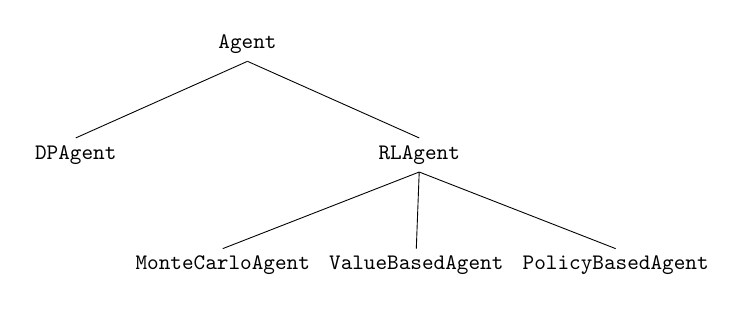
\begin{tikzpicture}[level distance=50,scale=0.8]
\Tree
[.\texttt{Agent}
    [.\texttt{DPAgent} ]
    [.\texttt{RLAgent}
        [.\texttt{MonteCarloAgent} ]
        [.\texttt{ValueBasedAgent} ]
        [.\texttt{PolicyBasedAgent} ]
    ]
]
\end{tikzpicture}
\caption{The agent hierarchy.}
\label{fig:agent_hierarchy}
\end{figure}

The actual implementations of the methods are in the \texttt{agents} directory. The reinforcement learning agents are trained through the \texttt{train()} method of the \texttt{RLAgent} class. In turn, this method repeatedly calls the \texttt{episode()} method, which trains the agent for one episode. In most cases, the implementation of the whole agent simply lies in the implementation of one episode of training.

The \texttt{core} folder also contains the implementation of the value functions (both state- and action-value functions, either represented by a matrix, or linearly approximated by a weight vector), the policies (a tabular one for dynamic programming, an implicitly derived one for value-based agents, and a parameterized one for policy-based agents), and the step size. The step size can be constant, linearly decaying, or exponentially decaying. The linearly decaying learning sequence of step sizes takes the form
\begin{equation}
    h_{\indexletter}\doteq\frac{h_{0}}{1+\left(d\cdot\indexletter\right)},
\end{equation}
where~${h_{0}}$ is some initial value,~${d}$ is a decay factor, and~${\indexletter}$ denotes the current episode. Unless otherwise noted, values of~${\robbinsmonro}$ (Robbins-Monro sequences of step sizes for value-based methods),~$\gradientstep$ (learning rate for gradient methods), and~${\varepsilon}$ (${\varepsilon}$-greedy policies) are computed using this definition.

\section{OpenAI Gym}
The environments are emulated using OpenAI Gym~{\cite{brockman2016gym}}, which is a suite of environments written in Python. We will now introduce it in brief.

Dynamic programming methods simply access the environment's dictionary \texttt{P} which, for each state and each possible action in that state, has a list of tuples, each containing:
\begin{enumerate*}[label=\arabic*)]
    \item the probability of transitioning to a certain next state;
    \item the next state in question;
    \item the reward associated with the transition;
    \item a boolean indicating whether a terminal state was reached.
\end{enumerate*}

In reinforcement learning methods the interaction between agent and environment takes place through the \texttt{step()} method, which accepts an action, and returns a tuple similar to the previous, without the transition probability, and the addition of a boolean indicating whether the execution of the environment was truncated (generally because of a time limit).

When an environment has terminated it can be reset to its initial state via the \texttt{reset()} method. Additionally, the environment can be rendered visually with the \texttt{render()} method. The environments can also be customized by setting a predefined wrapper class as parent of our class. For example, this has been used to implement both discretized and featurized states.

\end{appendices}
\bibliographystyle{unsrt}
\bibliography{bib}

\end{document}
